\section{Dokumentenelemente}
Neben dem Text gibt es noch weitere Elemente, die in einem Dokument vorkommen können. Dazu gehören unter anderem Bilder, Tabellen, Listen und Quellcode. In diesem Kapitel werden die wichtigsten Elemente vorgestellt.

\subsection{Listen}
In \LaTeX{} gibt es verschiedene Arten von Listen. Es folgen die wichtigsten Beispiele.

\subsubsection{Aufzählungen / ungeordnete Listen}

\begin{minipage}{0.58\textwidth}
    \begin{lstlisting}[language={[LaTeX]TeX}]
\begin{itemize}
    \item Erster Punkt
    \item Zweiter Punkt
    \item Dritter Punkt
\end{itemize}
\end{lstlisting}
\end{minipage}
\hfill
\begin{minipage}{0.35\textwidth}
    \begin{itemize}
        \item Erster Punkt
        \item Zweiter Punkt
        \item Dritter Punkt
    \end{itemize}
\end{minipage}

\subsubsection{Nummerierungen / geordnete Listen}

\begin{minipage}{0.58\textwidth}
    \begin{lstlisting}[language={[LaTeX]TeX}]
\begin{enumerate}
    \item Erster Punkt
    \item Zweiter Punkt
    \item Dritter Punkt
\end{enumerate}
\end{lstlisting}
\end{minipage}
\hfill
\begin{minipage}{0.35\textwidth}
    \begin{enumerate}
        \item Erster Punkt
        \item Zweiter Punkt
        \item Dritter Punkt
    \end{enumerate}
\end{minipage}

Falls die Nummerierung mit römischen Zahlen erfolgen soll, kann dies durch den Befehl \textbf{\texttt{\textbackslash begin\{enumerate\}[label=\textbackslash Roman*]}} erreicht werden. Analog dazu können für kleine römische Zahlen \textbf{\texttt{\textbackslash roman*}} und für Buchstaben \textbf{\texttt{\textbackslash alph*}} verwendet werden. Für diese Anpassungen wird das Paket \texttt{enumitem} benötigt.

\subsubsection{Definitionslisten}

\begin{minipage}{0.58\textwidth}
    \begin{lstlisting}[language={[LaTeX]TeX}]
\begin{description}
    \item[Erster Punkt] Beschreibung 1
    \item[Zweiter Punkt] Beschreibung 2
    \item[Dritter Punkt] Beschreibung 3
\end{description}
\end{lstlisting}
\end{minipage}
\hfill
\begin{minipage}{0.35\textwidth}
    \begin{description}
        \item[Erster Punkt] Beschreibung 1
        \item[Zweiter Punkt] Beschreibung 2
        \item[Dritter Punkt] Beschreibung 3
    \end{description}
\end{minipage}

\subsubsection{Angepasste Listen}

\begin{minipage}{0.58\textwidth}
    \begin{lstlisting}[language={[LaTeX]TeX}]
\begin{itemize}[label=$\rightarrow$]
    \item Erster Punkt
    \item Zweiter Punkt
    \item Dritter Punkt
\end{itemize}
\end{lstlisting}
\end{minipage}
\hfill
\begin{minipage}{0.35\textwidth}
    \begin{itemize}[label=$\rightarrow$]
        \item Erster Punkt
        \item Zweiter Punkt
        \item Dritter Punkt
    \end{itemize}
\end{minipage}

Neben $\rightarrow$ können auch andere Symbole oder Zeichenketten als Aufzählungszeichen verwendet werden. Es ist allerdings darauf zu achten ggf. (\$) für Objekte aus der Mathematikumgebung zu verwenden. Vorstellbar wären beispielsweise ein Haken $\checkmark$ (\$\textbackslash checkmark\$) oder ein Kreuz $\times$ (\$\textbackslash times\$). Es wird das Paket \texttt{enumitem} benötigt.

\subsubsection{Mehrspaltige Listen}

\begin{minipage}{0.50\textwidth}
    \begin{lstlisting}[language={[LaTeX]TeX}]
\begin{multicols}{2}
\begin{itemize}
    \item Erster Punkt
    \item Zweiter Punkt
    \item Dritter Punkt
    \item Vierter Punkt
\end{itemize}
\end{multicols}
\end{lstlisting}
\end{minipage}
\hfill
\begin{minipage}{0.48\textwidth}
    \begin{multicols}{2}
        \begin{itemize}
            \item Erster Punkt
            \item Zweiter Punkt
            \item Dritter Punkt
            \item Vierter Punkt
        \end{itemize}
    \end{multicols}
\end{minipage}

Mit der Umgebung \texttt{multicols} können mehrspaltige Listen erstellt werden. Die Anzahl der Spalten wird als Argument in geschweiften Klammern übergeben. Es wird das Paket \texttt{multicol} benötigt.

\subsection{Gleichungen / Mathematikumgebungen}
In \LaTeX{} gibt es verschiedene Umgebungen, um mathematische Formeln zu setzen. Die wichtigsten Aspekte zu den mathematischen Umgebungen werden im Folgenden vorgestellt.

\subsubsection{Inline-Gleichungen}
In einem Text können mathematische Formeln direkt eingebettet werden. Dazu wird der Text in zwei Dollarzeichen (\$) eingeschlossen.
Beispiel: $a^2 + b^2 = c^2$ (Syntax: \texttt{\$a\^{}2 + b\^{}2 = c\^{}2\$})

\subsubsection{Abgesetzte Gleichungen}
Für abgesetzte Gleichungen gibt es die Umgebung \textbf{\texttt{equation}}. Diese setzt die Gleichung zentriert und nummeriert sie.
Wird in der \textbf{\texttt{equation}}-Umgebung ein \textbf{\texttt{\textbackslash label\{...\}}} Befehl verwendet, kann die Gleichung im Text referenziert werden (\autoref{eq:planck}) (siehe auch: \nameref{sec:querverweise}).
Alternativ kann ebenfalls die Kurzform \textbf{\texttt{\textbackslash [ ... \textbackslash ]}} verwendet werden, bei welcher jedoch keine Nummerierung erfolgt.

\begin{minipage}{0.5\textwidth}
    \begin{lstlisting}[language={[LaTeX]TeX}]
\begin{equation}
    \label{eq:planck}
    E = h \cdot f
\end{equation}

\[
    E = h \cdot f
\]

\end{lstlisting}
\end{minipage}
\hfill
\begin{minipage}{0.5\textwidth}
    \begin{equation}
        \label{eq:planck}
        E = h \cdot f
    \end{equation}

    \[
        E = h \cdot f
    \]
\end{minipage}
Alternativ kann die Nummerierung unterdrückt werden, indem die \textbf{\texttt{equation*}}-Umgebung verwendet wird oder in dem der Befehl \textbf{\texttt{\textbackslash nonumber}} eingesetzt wird.

Darüber hinaus können die Gleichungsnummern mit \textbf{\texttt{\textbackslash tag\{...\}}} manuell gesetzt oder angepasst werden werden.

\begin{minipage}{0.5\textwidth}
    \begin{lstlisting}[language={[LaTeX]TeX}]
\begin{equation}
    \tag{Ladung}
    Q = \int I \, dt
\end{equation}
\end{lstlisting}
\end{minipage}
\hfill
\begin{minipage}{0.5\textwidth}
    \begin{equation}
        \tag{Ladung}
        Q = \int I \, dt
    \end{equation}
\end{minipage}

\subsubsection{Mehrzeilige Gleichungen}
Für mehrzeilige Gleichungen gibt es die \textbf{\texttt{align}}-Umgebung. Mit dem \textbf{\texttt{\&}}-Zeichen wird die Ausrichtung der Gleichungen festgelegt. Mit dem \textbf{\texttt{\textbackslash\textbackslash}}-Zeichen wird eine neue Zeile begonnen. Die Gleichungen werden an den \textbf{\texttt{\&}}-Zeichen ausgerichtet.

\begin{lstlisting}[language={[LaTeX]TeX}]
\begin{align}
    \label{eq:trig}
    1                 & = \sin^2{(x)} + \cos^2{(x)}     \\
    \label{eq:euler}
    \exp{(j \cdot x)} & = \cos{(x)} + j \cdot \sin{(x)}
\end{align}
\end{lstlisting}

\begin{align}
    \label{eq:trig}
    1                 & = \sin^2{(x)} + \cos^2{(x)}     \\
    \label{eq:euler}
    \exp{(j \cdot x)} & = \cos{(x)} + j \cdot \sin{(x)}
\end{align}

In den \textbf{\texttt{align}}-Umgebungen können die Gleichungen mit \textbf{\texttt{\textbackslash label\{...\}}} versehen werden, um sie im Text referenzieren zu können (\autoref{eq:trig} und \autoref{eq:euler}). Soll die Nummerierung einer einzelnen Gleichung unterdrückt werden, kann dies mit \textbf{\texttt{\textbackslash nonumber}} erreicht werden oder durch das Verwenden von \textbf{\texttt{\textbackslash begin\{align*\}}}.

In der \textbf{\texttt{equation}}-Umgebung kann die Unterumgebung \textbf{\texttt{aligned}} verwendet werden, um mehrzeilige Gleichungen mit dem \textbf{\texttt{\&}}-Zeichen auszurichten. Diese werden standardmäßig nur mir einer Gleichungsnummer versehen.

\subsubsection{Umrahmte Gleichungen}
Umrahmte Gleichungen können in \LaTeX{} mit dem \textbf{\texttt{boxed\{\}}}-Befehl erstellt werden. Dieser kann in den meisten mathematischen Umgebungen verwendet werden.

\begin{minipage}{0.5\textwidth}
    \begin{lstlisting}[language={[LaTeX]TeX}]
\begin{equation}
    \boxed{
    \begin{aligned}
        P &= U \cdot I \\
        &= I^2 \cdot R \\
        &= \frac{U^2}{R}
    \end{aligned}
    }
\end{equation}
\end{lstlisting}
\end{minipage}
\hfill
\begin{minipage}{0.5\textwidth}
    \begin{equation}
        \boxed{
            \begin{aligned}
                P & = U \cdot I     \\
                  & = I^2 \cdot R   \\
                  & = \frac{U^2}{R}
            \end{aligned}
        }
    \end{equation}
\end{minipage}




\subsubsection{Formatierung in Gleichungen}
In mathematischen Umgebungen können verschiedene Formatierungen vorgenommen werden. Dazu gehören unter anderem:

\begin{table}[h]
    \centering
    \renewcommand{\arraystretch}{1.3}
    \begin{tabular}{lll}
        \toprule
        \textbf{Formatierung}                & \textbf{LaTeX-Code}                                 & \textbf{Beispiel}        \\
        \midrule
        Fette Symbole (kann mehr als mathbf) & \texttt{\textbackslash bm\{\textbackslash varphi\}} & \( \bm{\varphi} \)       \\
        Fette Buchstaben                     & \texttt{\textbackslash mathbf\{x\}}                 & \( \mathbf{x} \)         \\
        Serifenlose Schrift                  & \texttt{\textbackslash mathsf\{x\}}                 & \( \mathsf{x} \)         \\
        Monospace (Typewriter)               & \texttt{\textbackslash mathtt\{x\}}                 & \( \mathtt{x} \)         \\
        Kursive Schrift                      & \texttt{\textbackslash mathit\{x\}}                 & \( \mathit{x} \)         \\
        Normale Schrift (Roman)              & \texttt{\textbackslash mathrm\{sin\}}               & \( \mathrm{sin} x \)     \\
        \midrule
        Durchgestrichen                      & \texttt{\textbackslash cancel\{x\}}                 & \( \cancel{x} \)         \\
        Unterstrichen                        & \texttt{\textbackslash underline\{x\}}              & \( \underline{x} \)      \\
        Überstrichen                         & \texttt{\textbackslash overline\{x\}}               & \( \overline{x} \)       \\
        \midrule
        Text in Mathemodus                   & \texttt{\textbackslash text\{Text\}}                & \( \text{Text} \)        \\
        \midrule
        Farbige Schrift (rot)                & \texttt{\textbackslash textcolor\{red\}\{x\}}       & \( \textcolor{red}{x} \) \\
        Farbige Gleichung (blau)             & \texttt{\textbackslash color\{blue\} x = 5}         & \( \color{blue} x = 5 \) \\
        \midrule
        Leerzeichen                          & \texttt{a b}                                        & \( a  b \)               \\
        Kleiner Abstand                      & \texttt{a\textbackslash ,b}                         & \( a\,b \)               \\
        Mittlerer Abstand                    & \texttt{a\textbackslash :b}                         & \( a\: b \)              \\
        Großer Abstand                       & \texttt{a\textbackslash ;b}                         & \( a\;b \)               \\
        Sehr großer Abstand                  & \texttt{a\textbackslash quad b}                     & \( a \quad b \)          \\
        Extra großer Abstand                 & \texttt{a\textbackslash qquad b}                    & \( a \qquad b \)         \\
        Negativer Abstand                    & \texttt{a\textbackslash!b}                          & \( a\!b \)               \\
        \bottomrule
    \end{tabular}
    \caption{Formatierungsoptionen in Mathematikumgebungen}
    \label{tab:math_formatierung}
\end{table}



\subsubsection{Mathematische Symbole}
In \LaTeX{} gibt es viele mathematische Rechenoperatoren und Symbole, die mit folgenden Befehlen in mathematische Umgebungen eingefügt werden können:

\begin{table}[H]
    \centering
    \renewcommand{\arraystretch}{1.3}
    \begin{tabular}{lll}
        \toprule
        \textbf{Operator}       & \textbf{LaTeX-Code}                                                 & \textbf{Beispiel}          \\
        \midrule
        Gleichheit              & \texttt{=}                                                          & $ a = b $                  \\
        Ungleichheit            & \texttt{\textbackslash neq}                                         & $ a \neq b $               \\
        Größer als              & \texttt{>}                                                          & $ a > b $                  \\
        Kleiner als             & \texttt{<}                                                          & $ a < b $                  \\
        Größer-gleich           & \texttt{\textbackslash geq}                                         & $ a \geq b $               \\
        Kleiner-gleich          & \texttt{\textbackslash leq}                                         & $ a \leq b $               \\
        Plus                    & \texttt{+}                                                          & $ a + b $                  \\
        Minus                   & \texttt{-}                                                          & $ a - b $                  \\
        Mal (×)                 & \texttt{\textbackslash times}                                       & $ a \times b $             \\
        Mal (Punkt)             & \texttt{\textbackslash cdot}                                        & $ a \cdot b $              \\
        Geteilt (Bruch)         & \texttt{\textbackslash frac\{a\}\{b\}}                              & $ \frac{a}{b} $            \\
        Geteilt (÷)             & \texttt{\textbackslash div}                                         & $ a \div b $               \\
        Prozent                 & \texttt{\%}                                                         & $ 50\% $                   \\
        Summenzeichen           & \texttt{\textbackslash sum\_\{i=1\}\^{}\{n\} ...}                   & $ \sum_{i=1}^{n} ... $     \\
        Produktzeichen          & \texttt{\textbackslash prod\_\{i=1\}\^{}\{n\} ...}                  & $ \prod_{i=1}^{n} ... $    \\
        Integral                & \texttt{\textbackslash int\_\{a\}\^{}\{b\} f(x) \textbackslash, dx} & $ \int_{a}^{b} f(x) \,dx $ \\
        Wurzel                  & \texttt{\textbackslash sqrt\{x\}}                                   & $ \sqrt{x} $               \\
        n-te Wurzel             & \texttt{\textbackslash sqrt[n]\{x\}}                                & $ \sqrt[n]{x} $            \\
        Logarithmus             & \texttt{\textbackslash log{(x)}}                                    & $ \log{(x)} $              \\
        Natürlicher Logarithmus & \texttt{\textbackslash ln{(x)}}                                     & $ \ln{(x)} $               \\
        Exponentialfunktion     & \texttt{e\^{}x}, \texttt{\textbackslash exp{(x)}}                   & $ e^x, \exp{(x)} $         \\
        Sinus                   & \texttt{\textbackslash sin{(x)}}                                    & $ \sin{(x)} $              \\
        Kosinus                 & \texttt{\textbackslash cos{(x)}}                                    & $ \cos{(x)} $              \\
        Tangens                 & \texttt{\textbackslash tan{(x)}}                                    & $ \tan{(x)} $              \\
        Cotangens               & \texttt{\textbackslash cot{(x)}}                                    & $ \cot{(x)} $              \\
        Arkussinus              & \texttt{\textbackslash arcsin{(x)}}                                 & $ \arcsin{(x)} $           \\
        Arkuskosinus            & \texttt{\textbackslash arccos{(x)}}                                 & $ \arccos{(x)} $           \\
        Arkustangens            & \texttt{\textbackslash arctan{(x)}}                                 & $ \arctan{(x)} $           \\
        Modulo                  & \texttt{a \textbackslash bmod b}                                    & $ a \bmod b $              \\
        Konjunktion (UND)       & \texttt{\textbackslash wedge}                                       & $ A \wedge B $             \\
        Disjunktion (ODER)      & \texttt{\textbackslash vee}                                         & $ A \vee B $               \\
        Negation                & \texttt{\textbackslash neg}                                         & $ \neg A $                 \\
        Implikation             & \texttt{\textbackslash Rightarrow}                                  & $ A \Rightarrow B $        \\
        Äquivalenz              & \texttt{\textbackslash Leftrightarrow}                              & $ A \Leftrightarrow B $    \\
        Natürliche Zahlen       & \texttt{\textbackslash mathbb\{N\}}                                 & \( \mathbb{N} \)           \\
        Ganze Zahlen            & \texttt{\textbackslash mathbb\{Z\}}                                 & \( \mathbb{Z} \)           \\
        Rationale Zahlen        & \texttt{\textbackslash mathbb\{Q\}}                                 & \( \mathbb{Q} \)           \\
        Reelle Zahlen           & \texttt{\textbackslash mathbb\{R\}}                                 & \( \mathbb{R} \)           \\
        Komplexe Zahlen         & \texttt{\textbackslash mathbb\{C\}}                                 & \( \mathbb{C} \)           \\
        \bottomrule
    \end{tabular}
    \caption{Wichtige Rechenoperatoren und mathematische Symbole}
    \label{tab:operatoren}
\end{table}

Darüber hinaus gibt es noch viele weitere mathematische Symbole, die in der VSC-Umgebung einfach über die \LaTeX{}-Erweiterung eingefügt werden können.

\subsubsection{Matrizen}
Matrizen können in \LaTeX{} mit der \textbf{\texttt{bmatrix}}-Umgebung erstellt werden. Die Spalten werden durch \textbf{\texttt{\&}} und die Zeilen durch \textbf{\texttt{\textbackslash\textbackslash}} getrennt.

\begin{minipage}{0.5\textwidth}
    \begin{lstlisting}[language={[LaTeX]TeX}]
\begin{equation}
    \begin{bmatrix}
        1 & 2 & 3 \\
        4 & 5 & 6 \\
        7 & 8 & 9
    \end{bmatrix}
\end{equation}
\end{lstlisting}
\end{minipage}
\hfill
\begin{minipage}{0.5\textwidth}
    \begin{equation}
        \begin{bmatrix}
            1 & 2 & 3 \\
            4 & 5 & 6 \\
            7 & 8 & 9
        \end{bmatrix}
    \end{equation}
\end{minipage}

Anstelle der \textbf{\texttt{bmatrix}}-Umgebung können die Umgebungen \textbf{\texttt{pmatrix}} (runde Klammern), \textbf{\texttt{Bmatrix}} (geschweifte Klammern), \textbf{\texttt{vmatrix}} (einfache Striche) und \textbf{\texttt{Vmatrix}} (doppelte Striche) verwendet werden.

Die Determinante einer Matrix kann mit dem Befehl \textbf{\texttt{\textbackslash det}} gesetzt werden. Die Transponierte einer Matrix kann mit dem Befehl \textbf{\texttt{\textbackslash top}} und die Inverse einer Matrix kann folgendermaßen gesetzt werden:

\begin{minipage}{0.5\textwidth}
    \begin{lstlisting}[language={[LaTeX]TeX}]
\begin{equation}
    \det
    \begin{bmatrix}
        a & b \\
        c & d
    \end{bmatrix}^{-1}
\end{equation}
\end{lstlisting}
\end{minipage}
\hfill
\begin{minipage}{0.5\textwidth}
    \begin{equation}
        \det
        \begin{bmatrix}
            a & b \\
            c & d
        \end{bmatrix}^{-1}
    \end{equation}
\end{minipage}



\subsubsection{Fallunterscheidungen}
Fallunterscheidungen können in \LaTeX{} mit der \textbf{\texttt{cases}}-Umgebung erstellt werden. Die einzelnen Fälle werden durch \textbf{\texttt{\textbackslash\textbackslash}} getrennt und mit \textbf{\texttt{\&}} ausgerichtet.

\begin{minipage}{0.5\textwidth}
    \begin{lstlisting}[language={[LaTeX]TeX}]
\begin{equation}
    f(x) =
    \begin{cases}
        0 & \text{:\quad} x < 0 \\
        1 & \text{:\quad} x \geq 0
    \end{cases}
\end{equation}
\end{lstlisting}
\end{minipage}
\hfill
\begin{minipage}{0.5\textwidth}
    \begin{equation}
        f(x) =
        \begin{cases}
            0 & \text{:\quad} x < 0    \\
            1 & \text{:\quad} x \geq 0
        \end{cases}
    \end{equation}
\end{minipage}

\subsubsection{Gleichungssysteme}
Gleichungssysteme können in \LaTeX{} mit der \textbf{\texttt{gather}}-Umgebung erstellt werden. Die einzelnen Gleichungen werden durch \textbf{\texttt{\textbackslash\textbackslash}} getrennt.

\begin{minipage}{0.5\textwidth}
    \begin{lstlisting}[language={[LaTeX]TeX}]
\begin{gather}
    x + y = 1 \\
    2x - y = 3
\end{gather}
\end{lstlisting}
\end{minipage}
\hfill
\begin{minipage}{0.5\textwidth}
    \begin{gather}
        x + y = 1 \\
        2x - y = 3
    \end{gather}
\end{minipage}

\subsection{Quellcode}
Quellcode kann in \LaTeX{} mit der \textbf{\texttt{lstlisting}}-Umgebung eingefügt werden. Dabei können verschiedene Einstellungen vorgenommen werden, um den Quellcode optisch ansprechend darzustellen. Es wird das Paket \textbf{\texttt{listings}} mit der Option \textbf{\texttt{pmboxdraw}} benötigt.

Ein Quellcode-Block kann auf folgende Weise eingefügt werden:

\begin{minipage}{0.48\textwidth}
    \begin{verbatim}
\begin{lstlisting}[language=Python]
def fibonacci(n):
    a, b = 0, 1
    for _ in range(n):
        print(a)
        a, b = b, a + b
\end{lstlisting}
\end{verbatim}
\end{minipage}
\hfill
\begin{minipage}{0.48\textwidth}
    \begin{lstlisting}[language=Python]
def fibonacci(n):
    a, b = 0, 1
    for _ in range(n):
        print(a)
        a, b = b, a + b
    \end{lstlisting}
\end{minipage}

Die Sprache des Quellcode wird mit in dem Befehl \textbf{\texttt{\textbackslash begin\{lstlisting\}[language=...]}} angegeben. Es können verschiedene Sprachen wie Python, Java, C++ oder auch \LaTeX{} selbst verwendet werden.

\subsubsection{Einstellungen für Quellcode}
Die Einstellungen für die Darstellung des Quellcodes können in der Präambel des Dokuments vorgenommen werden.

\begin{lstlisting}[language={[LaTeX]TeX}]
\usepackage{listings, pmboxdraw}
\lstset{
    language={[LaTeX]TeX},              % Programmiersprache
    frame=single,                       % Rahmen um den Code
    numbers=left,                       % Zeilennummern links
    stepnumber=1,                       % Jede Zeile nummerieren
    lineskip=0pt,                       % Zeilenabstand anpassen
    numberstyle=\footnotesize,          % Kleine Zeilennummern
    basicstyle=\ttfamily,               % Monospace-Schriftart
    keywordstyle=\color{blue},          % Keywords blau
    commentstyle=\color{gray},          % Kommentare grau
    stringstyle=\color{green},          % Strings gruen
    backgroundcolor=\color{white},      % Hintergrundfarbe
    showstringspaces=false,             % Keine Leerzeichen in Strings
    captionpos=b,                       % Position unter dem Code 
    breaklines=true,                    % Zeilenumbruch
}
\end{lstlisting}

\subsubsection{Farbliche Hervorhebung im Quellcode}
Soll in dem Code ein Zeile \textbf{farblich hervorgehoben} werden, kann dies mit dem Befehl \textbf{\texttt{\textbackslash begin\{lstlisting\}[language=..., emph=\{x,...\}, emphstyle=\{\textbackslash color\{red\}\}]}} erreicht werden. Dabei wird jedes x in dem Code rot hervorgehoben.

\begin{lstlisting}[language=C, emph={x}, emphstyle=\color{red}]
int main() {
    int x = 5;
    printf("X: %d\n", x);
}
\end{lstlisting}

\subsubsection{Beschriftung und Referenzierung des Quellcodes}
Gelegentlich ist es gewünscht ein eine Code-Box zu beschriften und sie referenzieren zu können. Dies kann mit dem Befehl \textbf{\texttt{\textbackslash begin\{lstlisting\}[language=C, caption=Beispielcode, label=scr:beispiel]}} erreicht werden (\autoref{scr:beispiel}) (siehe auch: \nameref{sec:querverweise}).

\begin{lstlisting}[language=C, caption=Beispielcode, label=scr:beispiel]
int bsp() {
    printf("Das ist ein Beispiel");
}   
\end{lstlisting}

\subsubsection{Externe Quellcode-Dateien einbinden}
In manchen Fällen kann es sinnvoll sein, den Quellcode aus einer externen Datei einzubinden. Dies kann mit dem Befehl \textbf{\texttt{\textbackslash lstinputlisting[Optionen]\{Pfad/zur/Datei.endung\}}} erreicht werden.

\lstinputlisting[language=C, caption=Beispielcode aus externer Datei, label=scr:extern]{anlagen/beispiel.c}

\subsection{Bilder}
In \LaTeX{} können Bilder auf folgende Weise eingefügt werden:
Es wird das Paket \textbf{\texttt{graphicx}} benötigt.

\begin{lstlisting}[language={[LaTeX]TeX}]
\begin{figure}[H]
    \centering
    \includegraphics[width=0.5\textwidth]{Pfad/zum/Bild.png}
    \caption{Bildunterschrift}
    \label{fig:bild}
\end{figure}
\end{lstlisting}

Ausschlaggebend für das Inkludieren ist der Befehl \textbf{\texttt{\textbackslash includegraphics[options]\{Pfad/zum/Bild.png\}}}.

Dabei können folgende Optionen verwendet werden:

\subsubsection{Optionen für \texttt{\textbackslash includegraphics}}
\begin{table}[H]
    \centering
    \begin{tabular}{lll}
        \toprule
        \textbf{Option} & \textbf{Wirkung}               & \textbf{Befehl}                               \\
        \midrule
        width           & Breite des Bildes              & \texttt{[width=5cm]}                          \\
        width           & Breite relativ zum Text        & \texttt{[width=0.5\textbackslash textwidth]}  \\
        height          & Höhe des Bildes                & \texttt{[height=4cm]}                         \\
        scale           & Skaliert das Bild              & \texttt{[scale=0.5]}                          \\
        angle           & Dreht das Bild um einen Winkel & \texttt{[angle=90]}                           \\
        origin          & Rotationspunkt ändern          & \texttt{[angle=90,origin=Rotationspunkt]}     \\
        clip            & Schneidet das Bild zu (in pt)  & \texttt{[clip,trim= links unten rechts oben]} \\
        draft           & Nur einen Platzhalterrahmen    & \texttt{[draft]}                              \\
        \bottomrule
    \end{tabular}
    \caption{Optionen für \texttt{\textbackslash includegraphics} in LaTeX}
    \label{tab:graphics_options}
\end{table}

\begin{figure}[H]
    \centering
    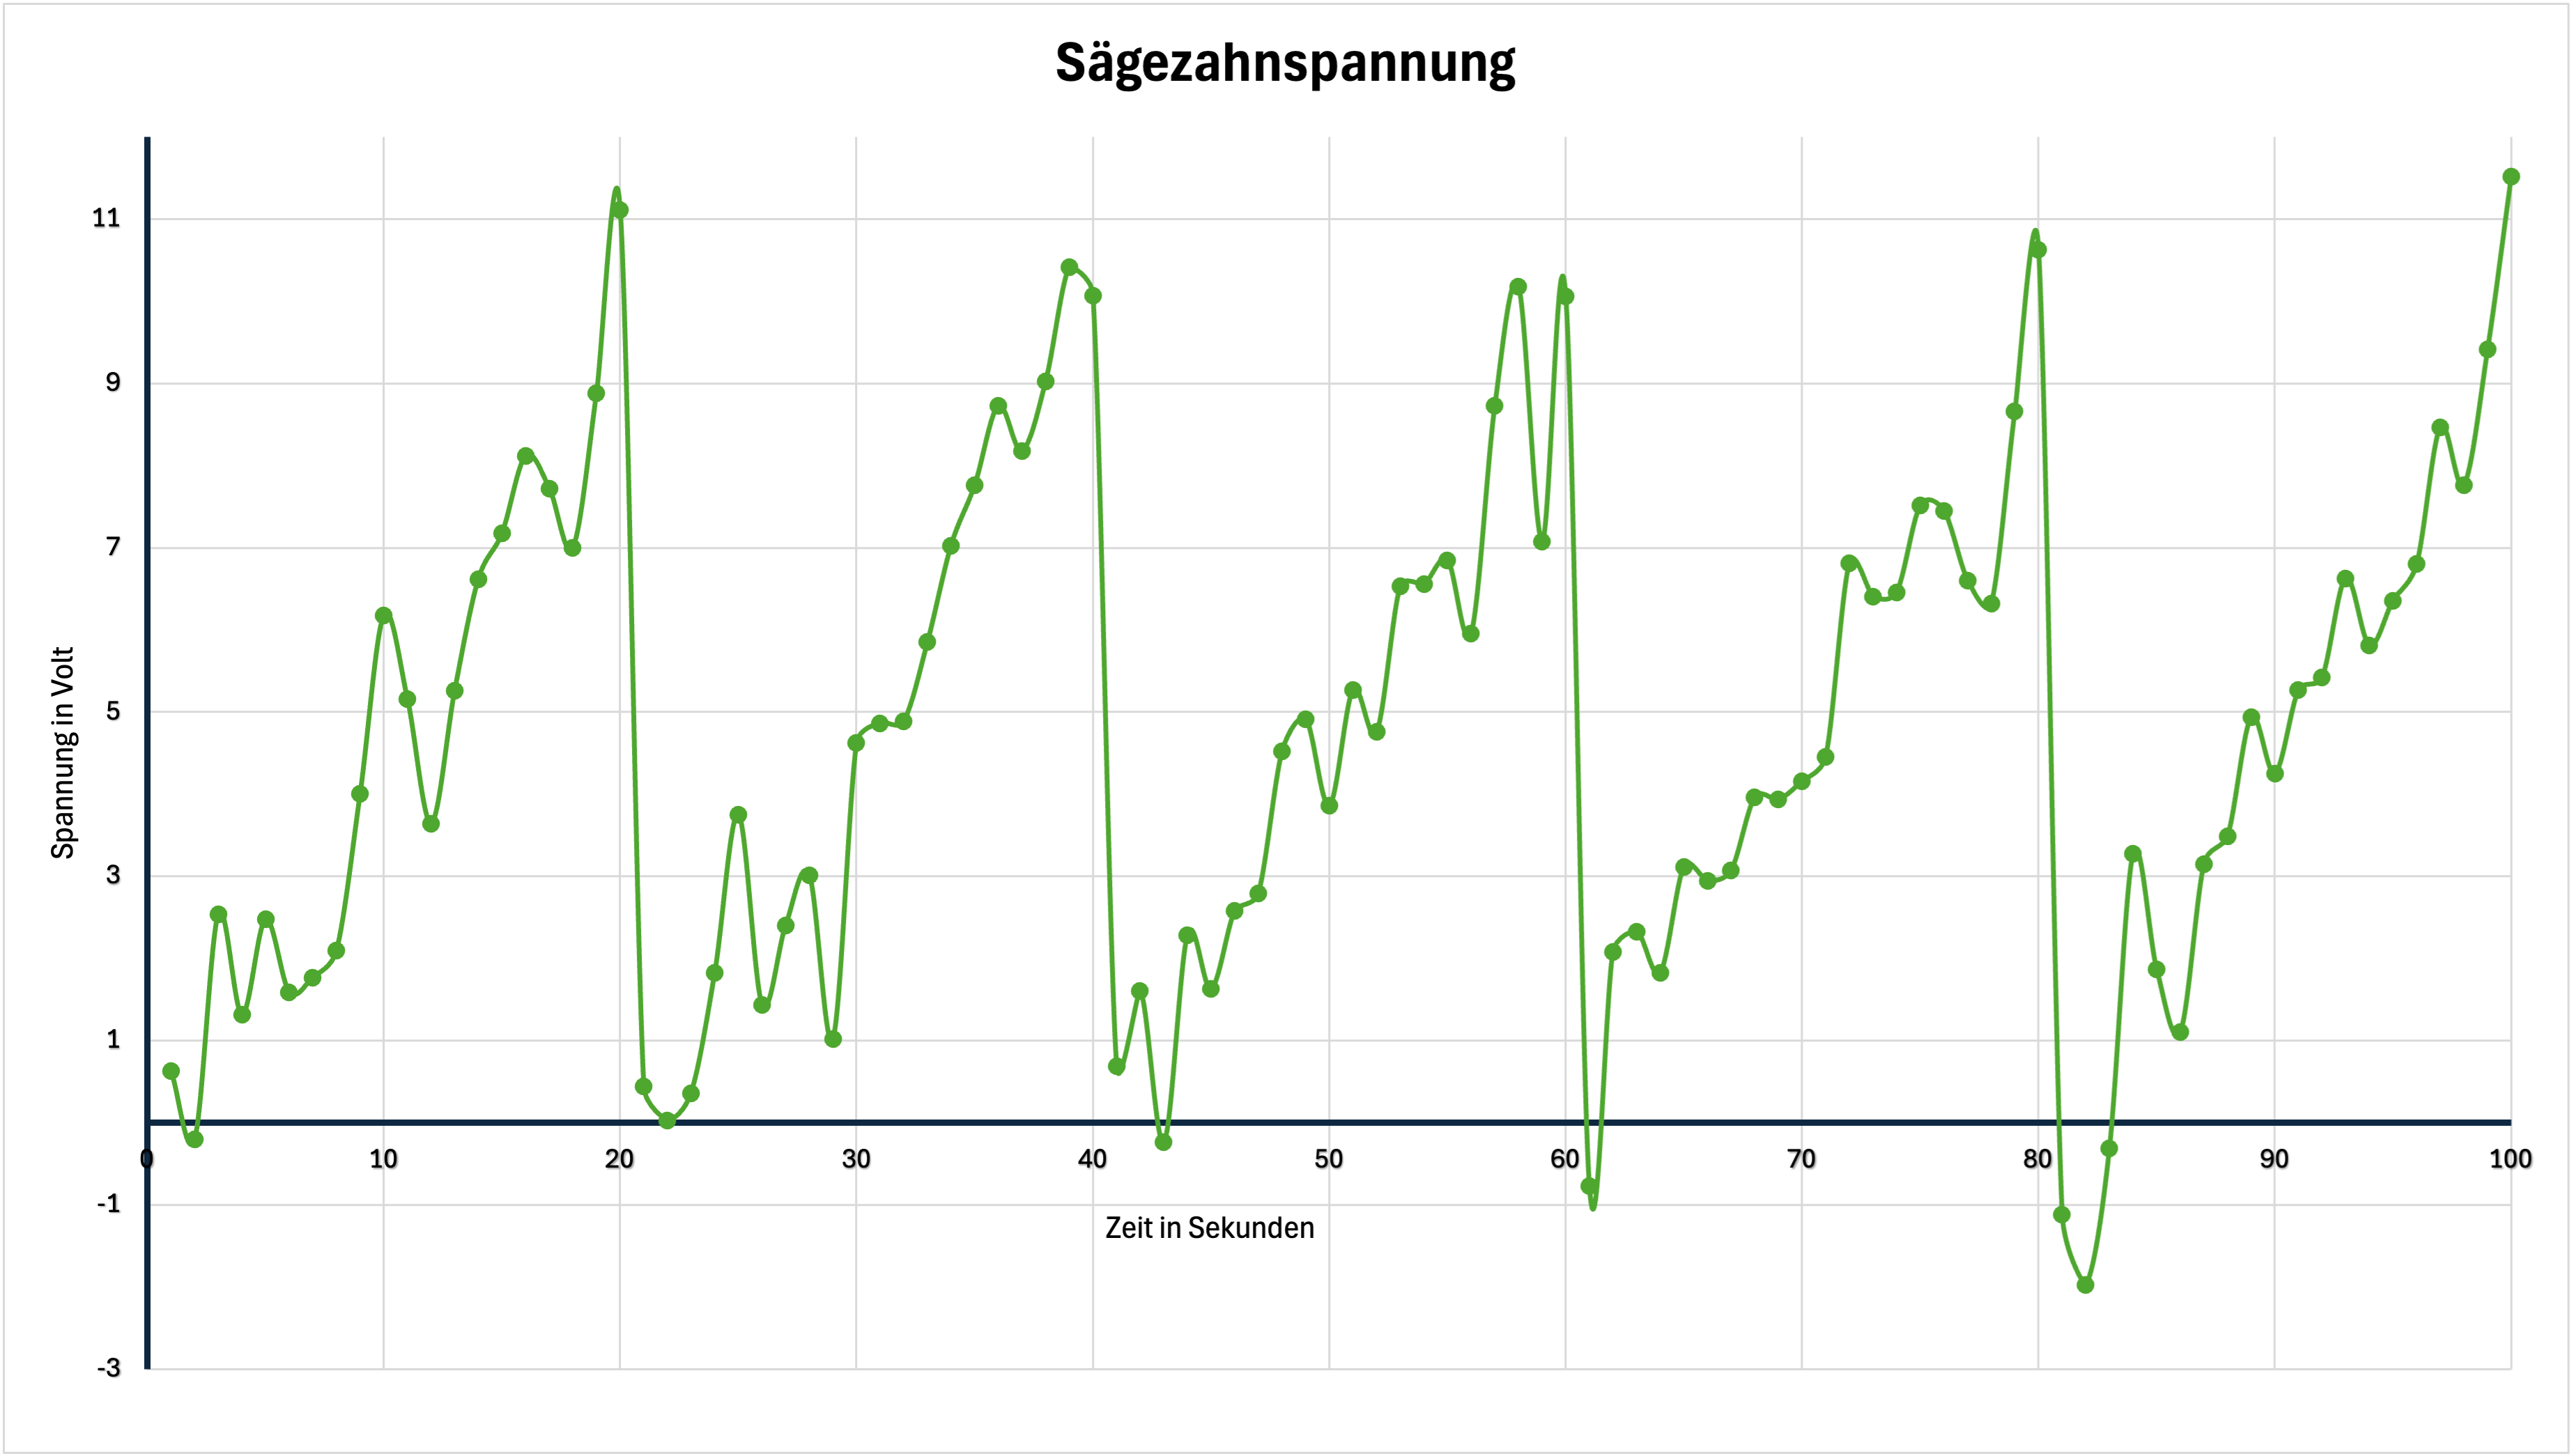
\includegraphics[width=0.7\textwidth]{anlagen/bilder/Graph.png}
    \caption{Sägezahnspannung}
    \label{fig:sägezahnspannung}
\end{figure}

Darüber hinaus können Bilder mit dem Befehl \texttt{\textbf{\textbackslash reflectbox\{\textbackslash includegraphics[...]\{Pfad/zum/Bild.png\}\}}} gespiegelt werden.

\subsubsection{Platzierung von Bildern}
Die Platzierung von Bildern kann mit den folgenden Optionen in \textbf{\texttt{\textbackslash begin\{figure\}[...]}} gesteuert werden.

\begin{table}[H]
    \centering
    \begin{tabular}{ll}
        \toprule
        \textbf{Option} & \textbf{Wirkung}               \\
        \midrule
        h               & Hier (here)                    \\
        t               & Oben (top)                     \\
        b               & Unten (bottom)                 \\
        p               & Auf einer eigenen Seite (page) \\
        H               & Genau hier (here)              \\
        \bottomrule
    \end{tabular}
    \caption{Platzierungsoptionen für Bilder, Tabellen und ähnliche Elemente}
    \label{tab:figure_options}
\end{table}

Für die H-Positionierungsoption wird das Paket \textbf{\texttt{float}} benötigt.

\subsubsection{Beschriftung und Referenzierung von Bildern}
Bilder können mit dem Befehl \textbf{\texttt{\textbackslash caption\{Bildunterschrift\}}} beschriftet werden. Mit dem Befehl \textbf{\texttt{\textbackslash label\{fig:bild\}}} wird ein Label gesetzt, auf welches im Text referenziert werden kann (\autoref{fig:sägezahnspannung})(siehe auch: \nameref{sec:querverweise}).

\subsubsection{Gerahmte Bilder}
Bilder können mit dem Befehl \textbf{\texttt{\textbackslash fbox\{\textbackslash includegraphics[...]\{Pfad/zum/Bild.png\}\}}} oder mit dem \textbf{\texttt{\textbackslash shadowbox\{\textbackslash includegraphics[...]\{Pfad/zum/Bild.png\}\}}} gerahmt werden. Für die Schattierung wird das Paket \textbf{\texttt{fancybox}} benötigt. Siehe auch \autoref{sec:rahmen_und_boxen}.

\begin{figure}[H]
    \centering
    \begin{subfigure}{0.45\textwidth}
        \centering
        \fbox{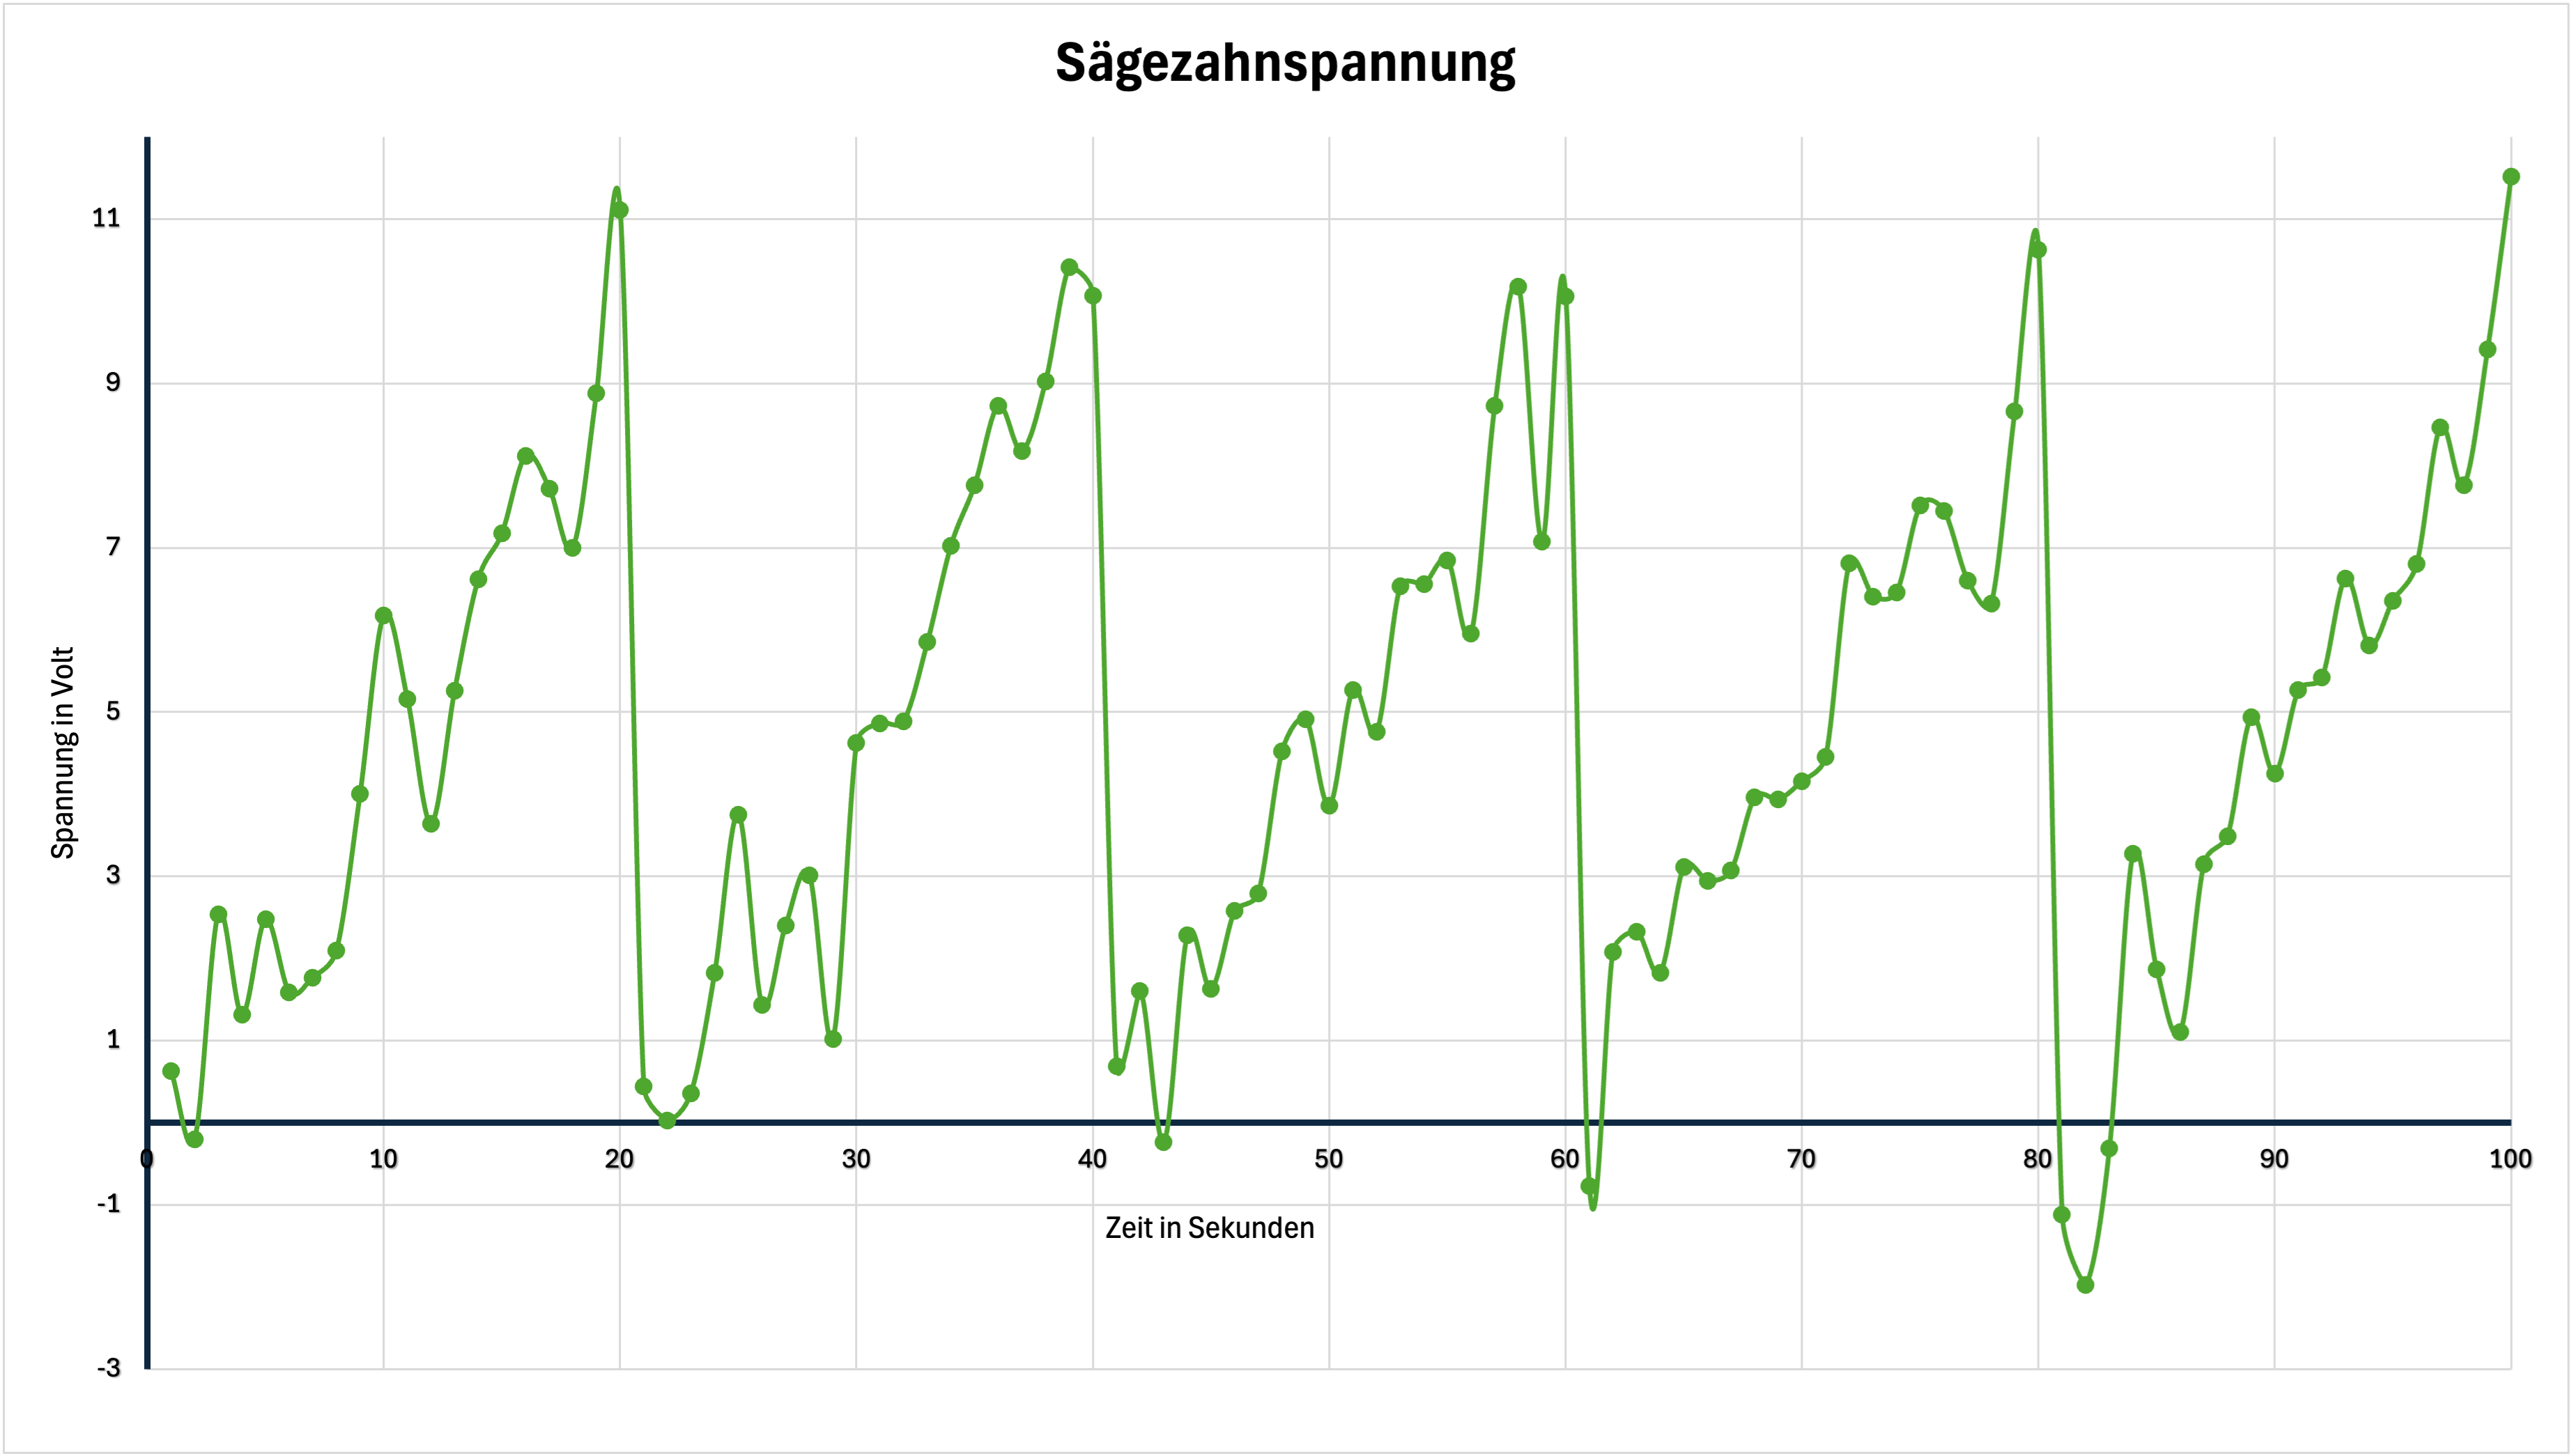
\includegraphics[width=0.9\textwidth]{anlagen/bilder/Graph.png}}
        \caption{Gerahmtes Bild}
        \label{fig:gerahmtes_bild}
    \end{subfigure}
    \hfill
    \begin{subfigure}{0.45\textwidth}
        \centering
        \shadowbox{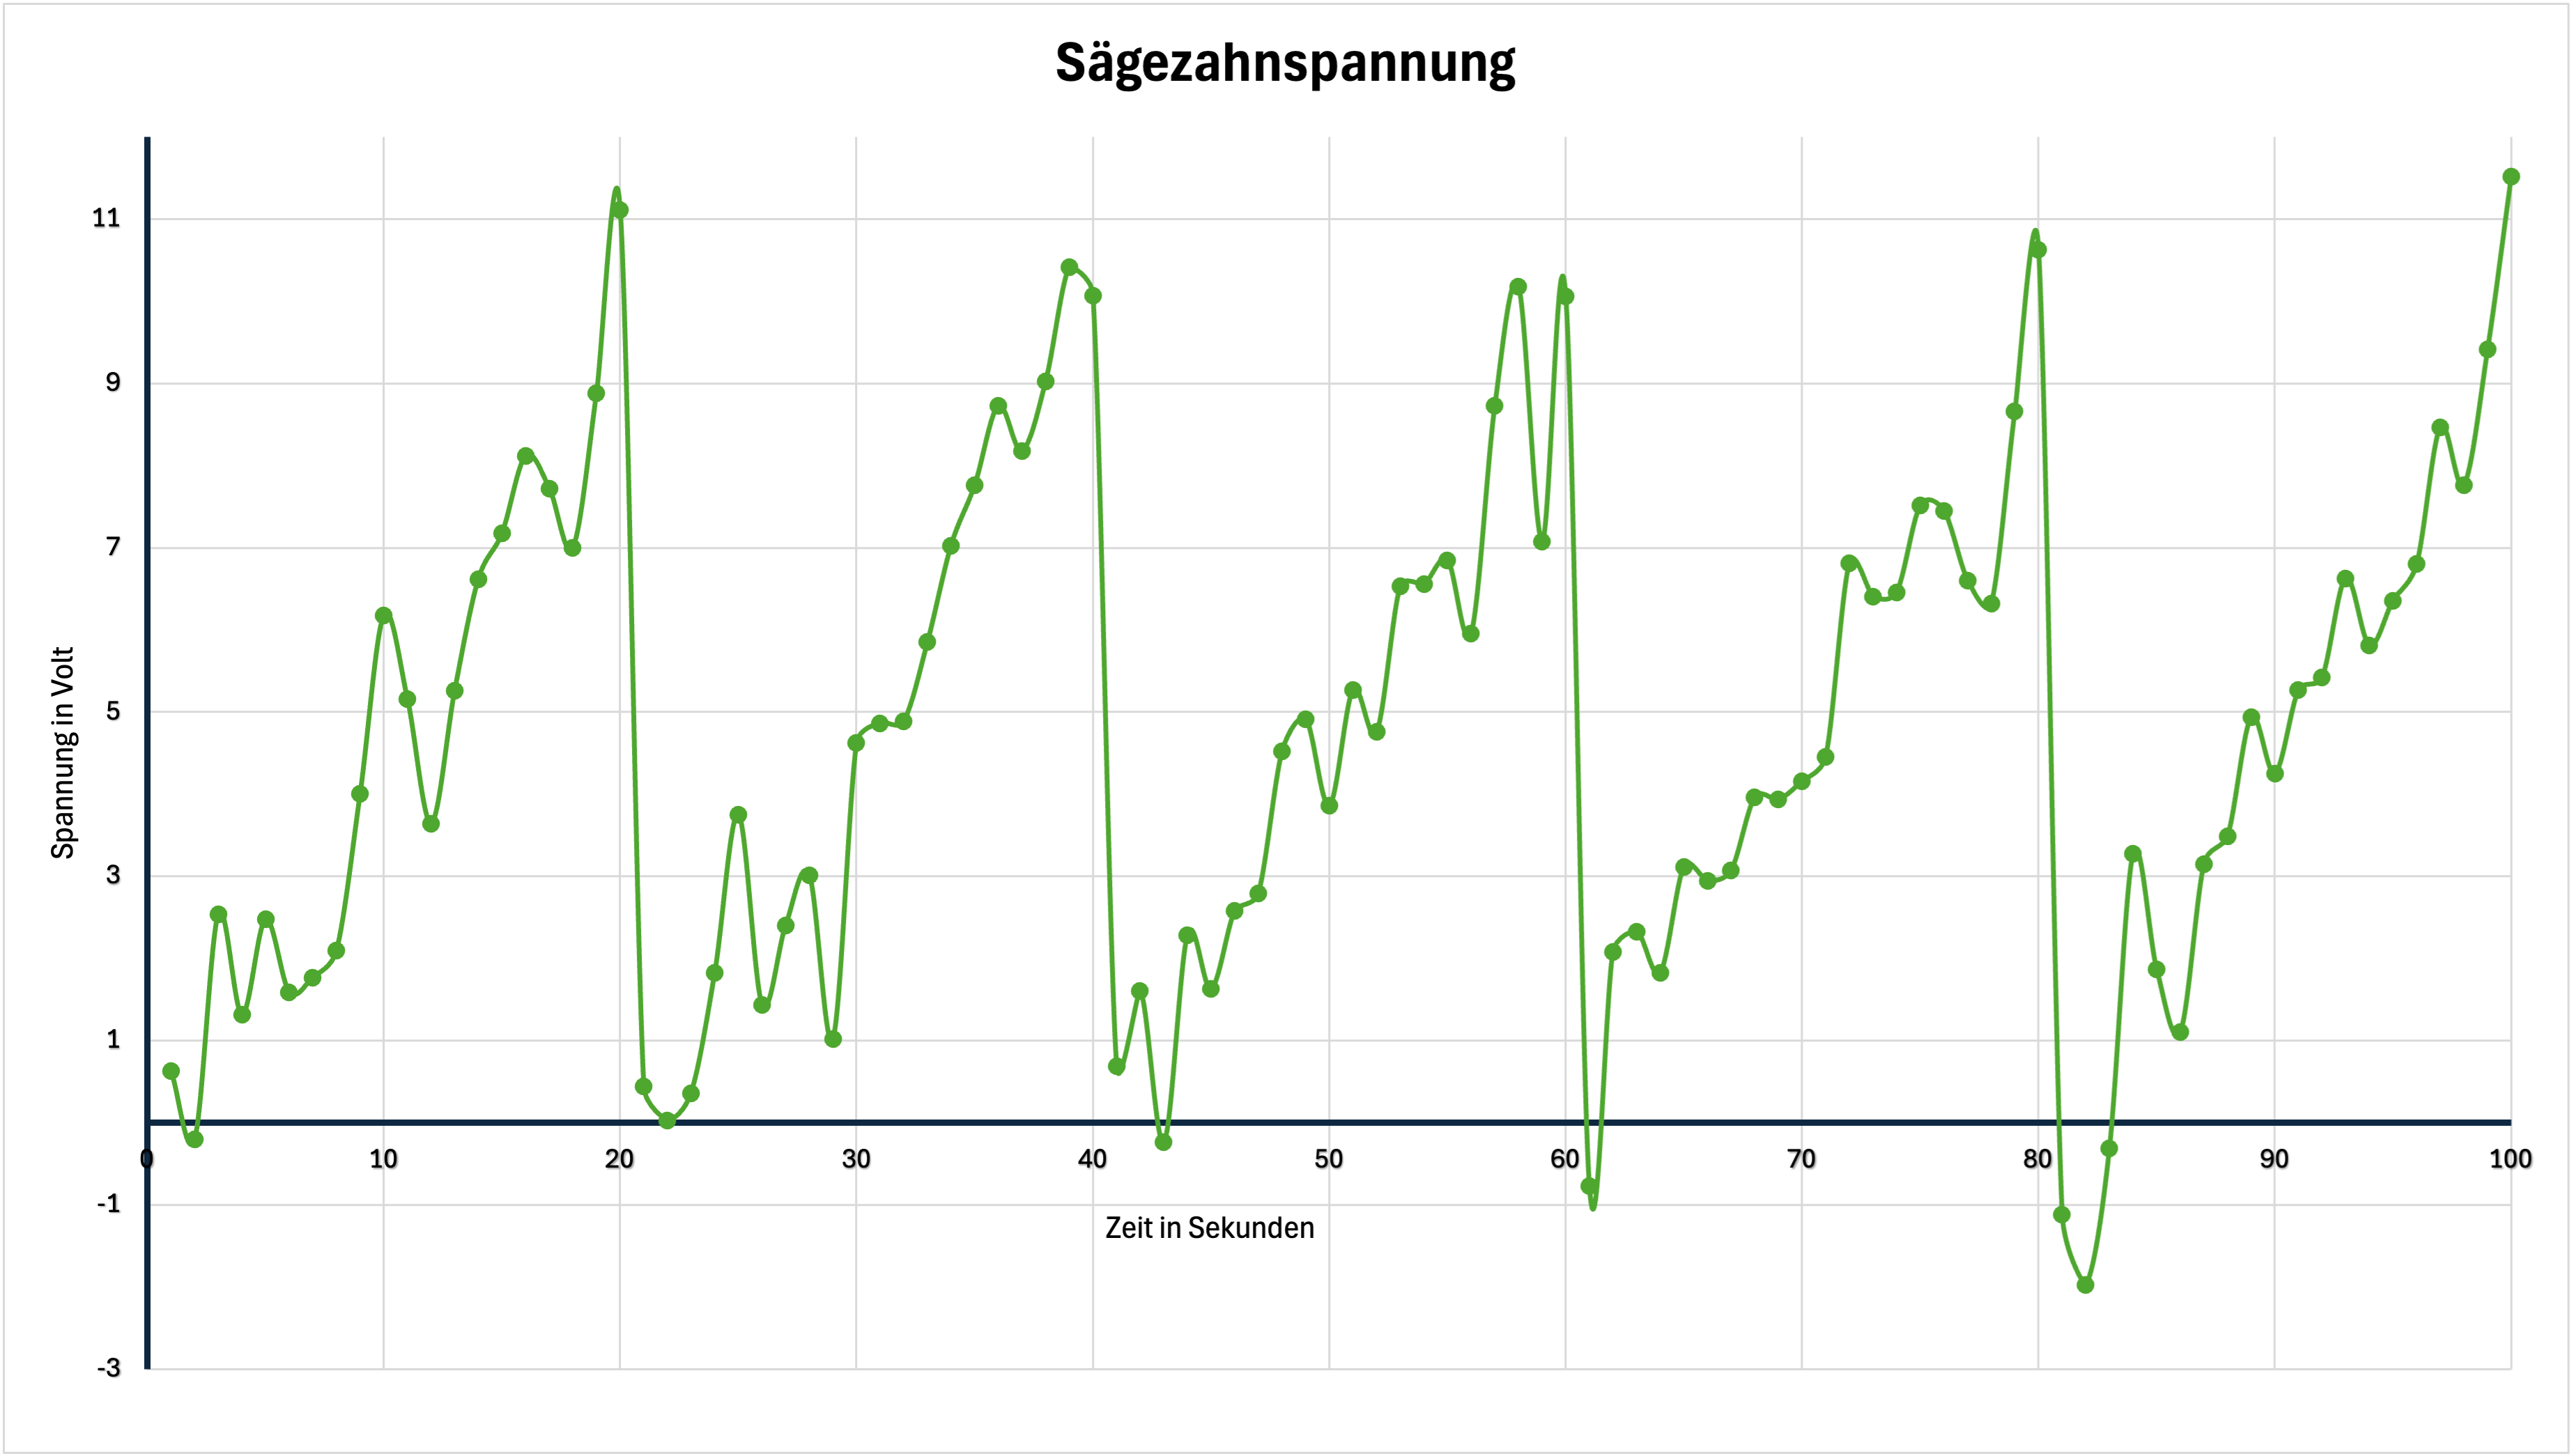
\includegraphics[width=0.9\textwidth]{anlagen/bilder/Graph.png}}
        \caption{Schattiertes Bild}
        \label{fig:schattiertes_bild}
    \end{subfigure}
    \caption{Gerahmte und schattierte Bilder}
    \label{fig:gerahmte_schattierte_bilder}
\end{figure}


\subsubsection{Parallele Darstellung von Bildern}
Mehrere Bilder können mit der \textbf{\texttt{subfigure}}-Umgebung in einer \textbf{\texttt{figure}}-Umgebung dargestellt werden. Dabei können die Bilder mit \textbf{\texttt{\textbackslash hfill}} horizontal nebeneinander platziert werden. Darüber hinaus ist die Darstellung von mehreren Bildern in einer \textbf{\texttt{minipage}}-Umgebung möglich (siehe auch: \nameref{sec:minipage}).

\begin{lstlisting}[language={[LaTeX]TeX}]
\begin{figure}[H]
    \centering
    \begin{subfigure}{0.45\textwidth}
        \centering
        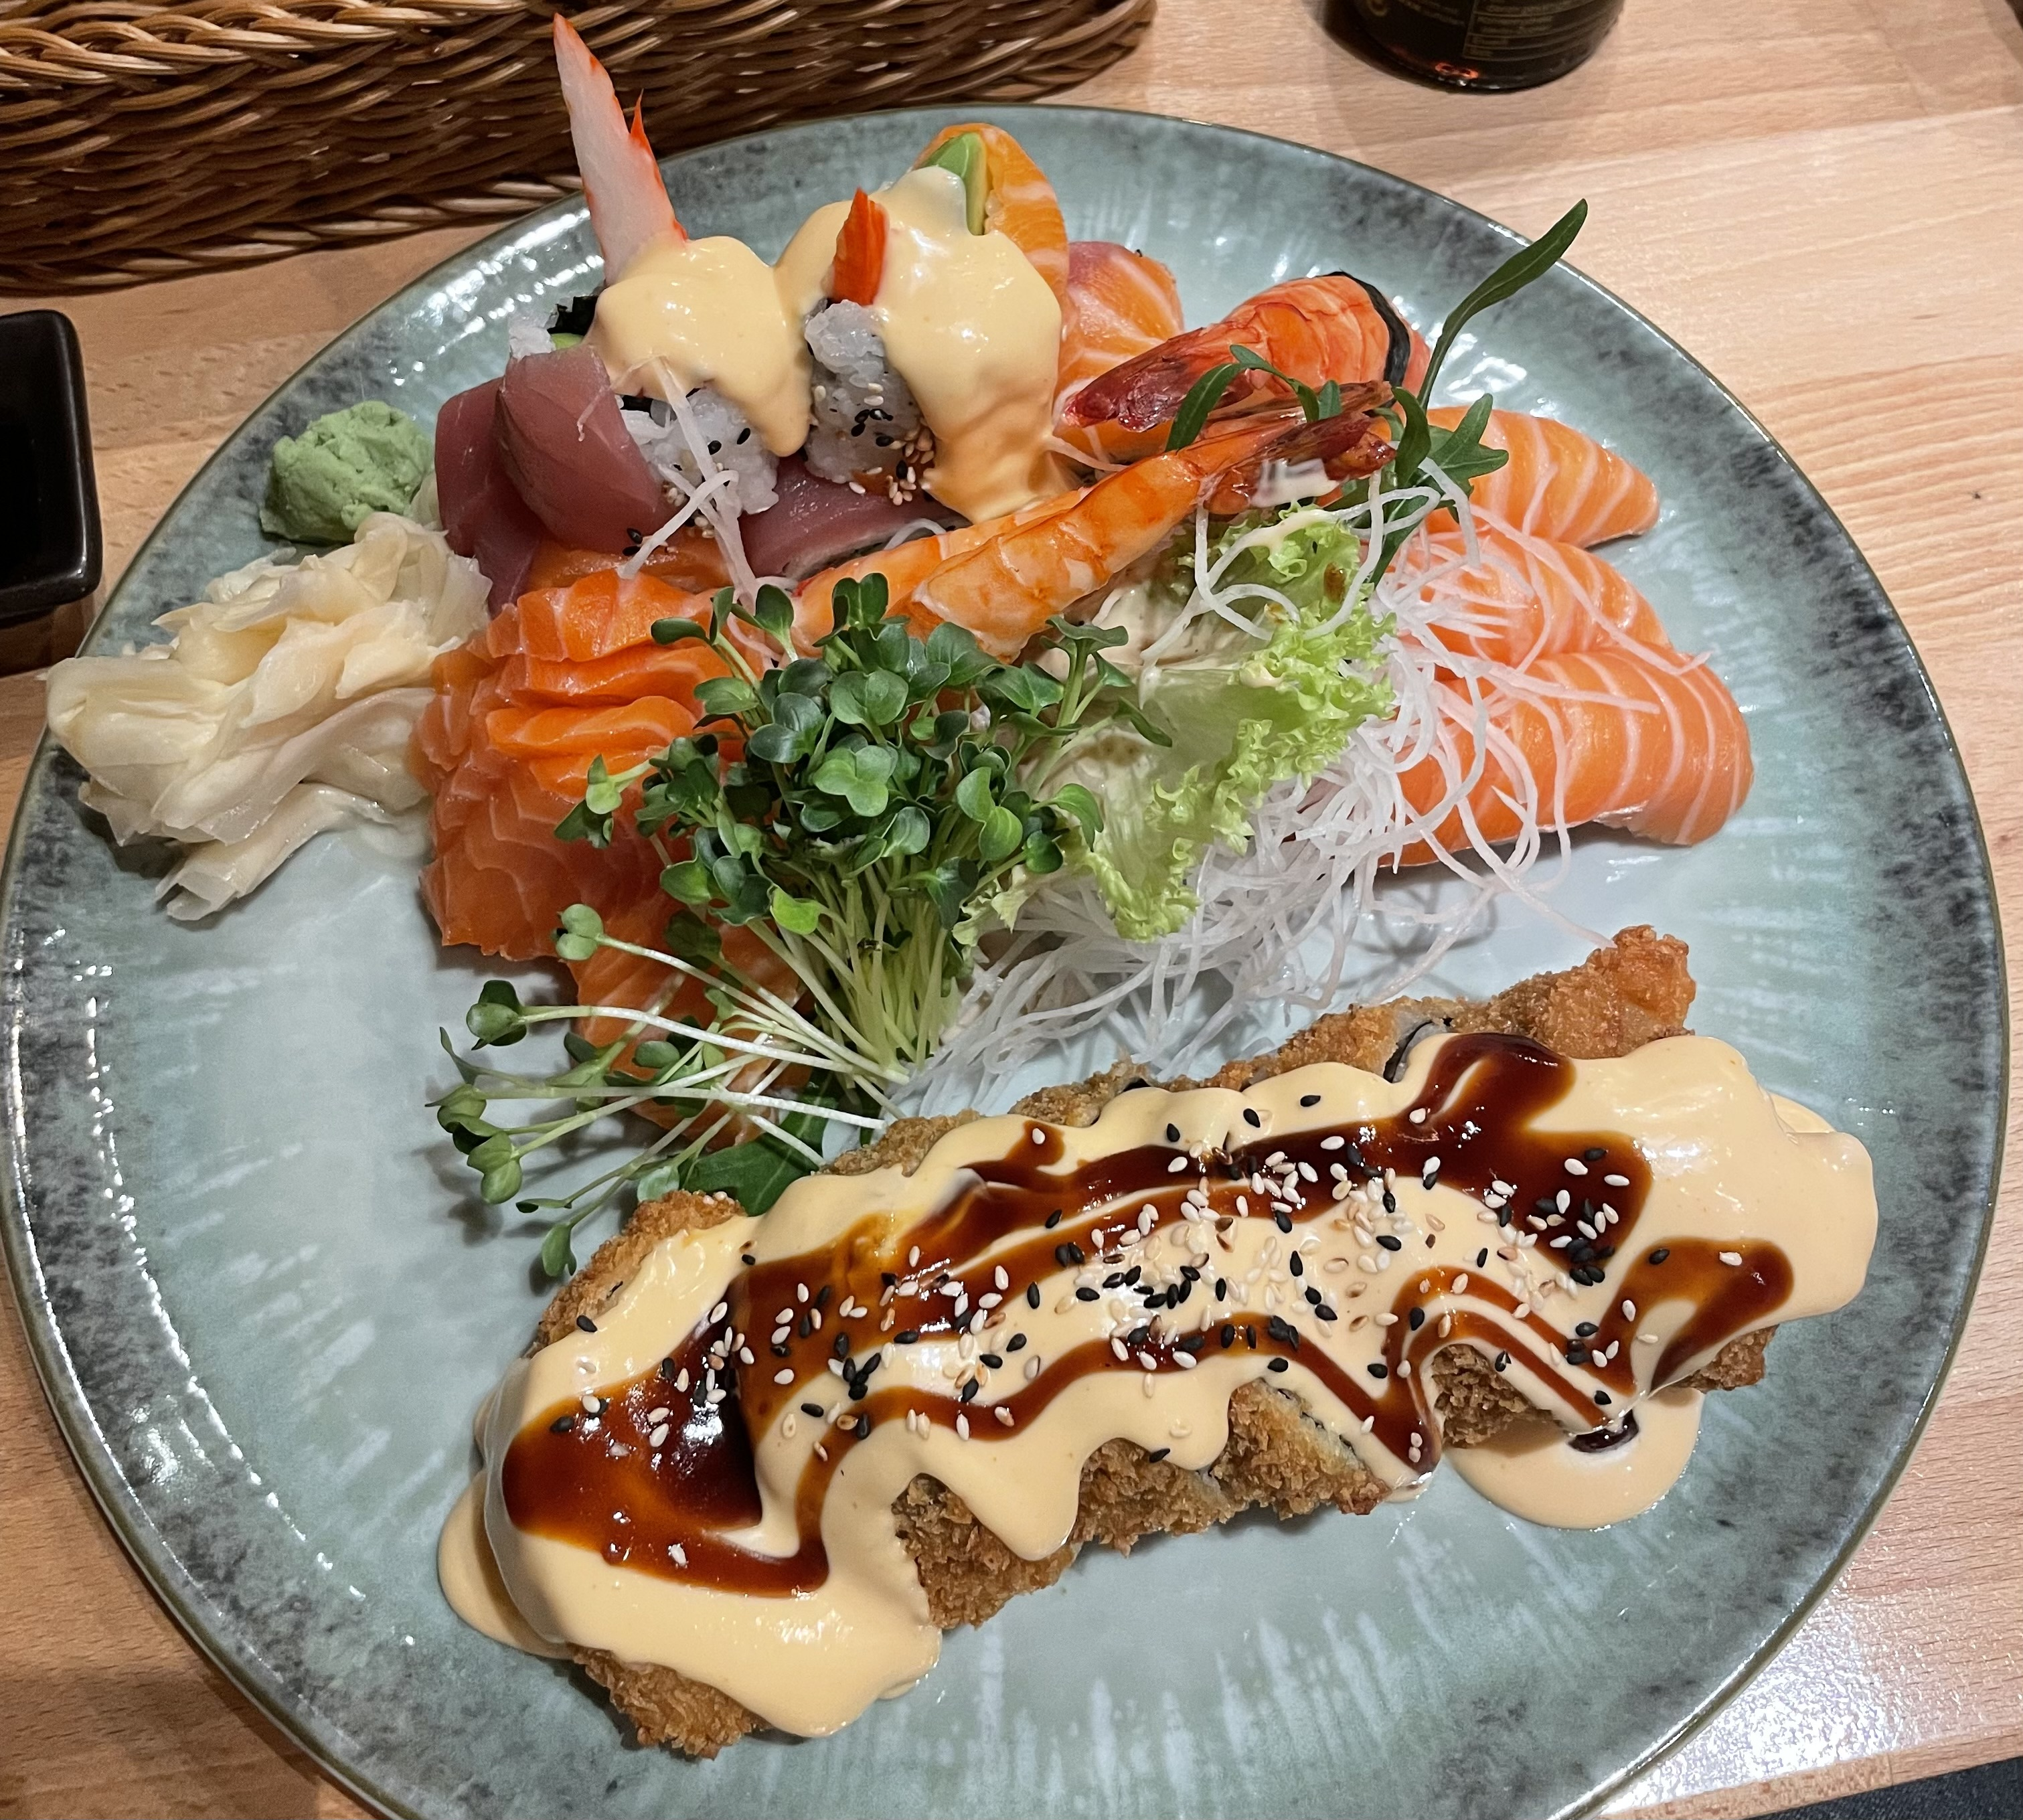
\includegraphics[width=0.9\textwidth]{anlagen/bilder/Bild1.jpg}
        \caption{Bild 1}
        \label{fig:bild1}
    \end{subfigure}
    \hfill
    \begin{subfigure}{0.45\textwidth}
        \centering
        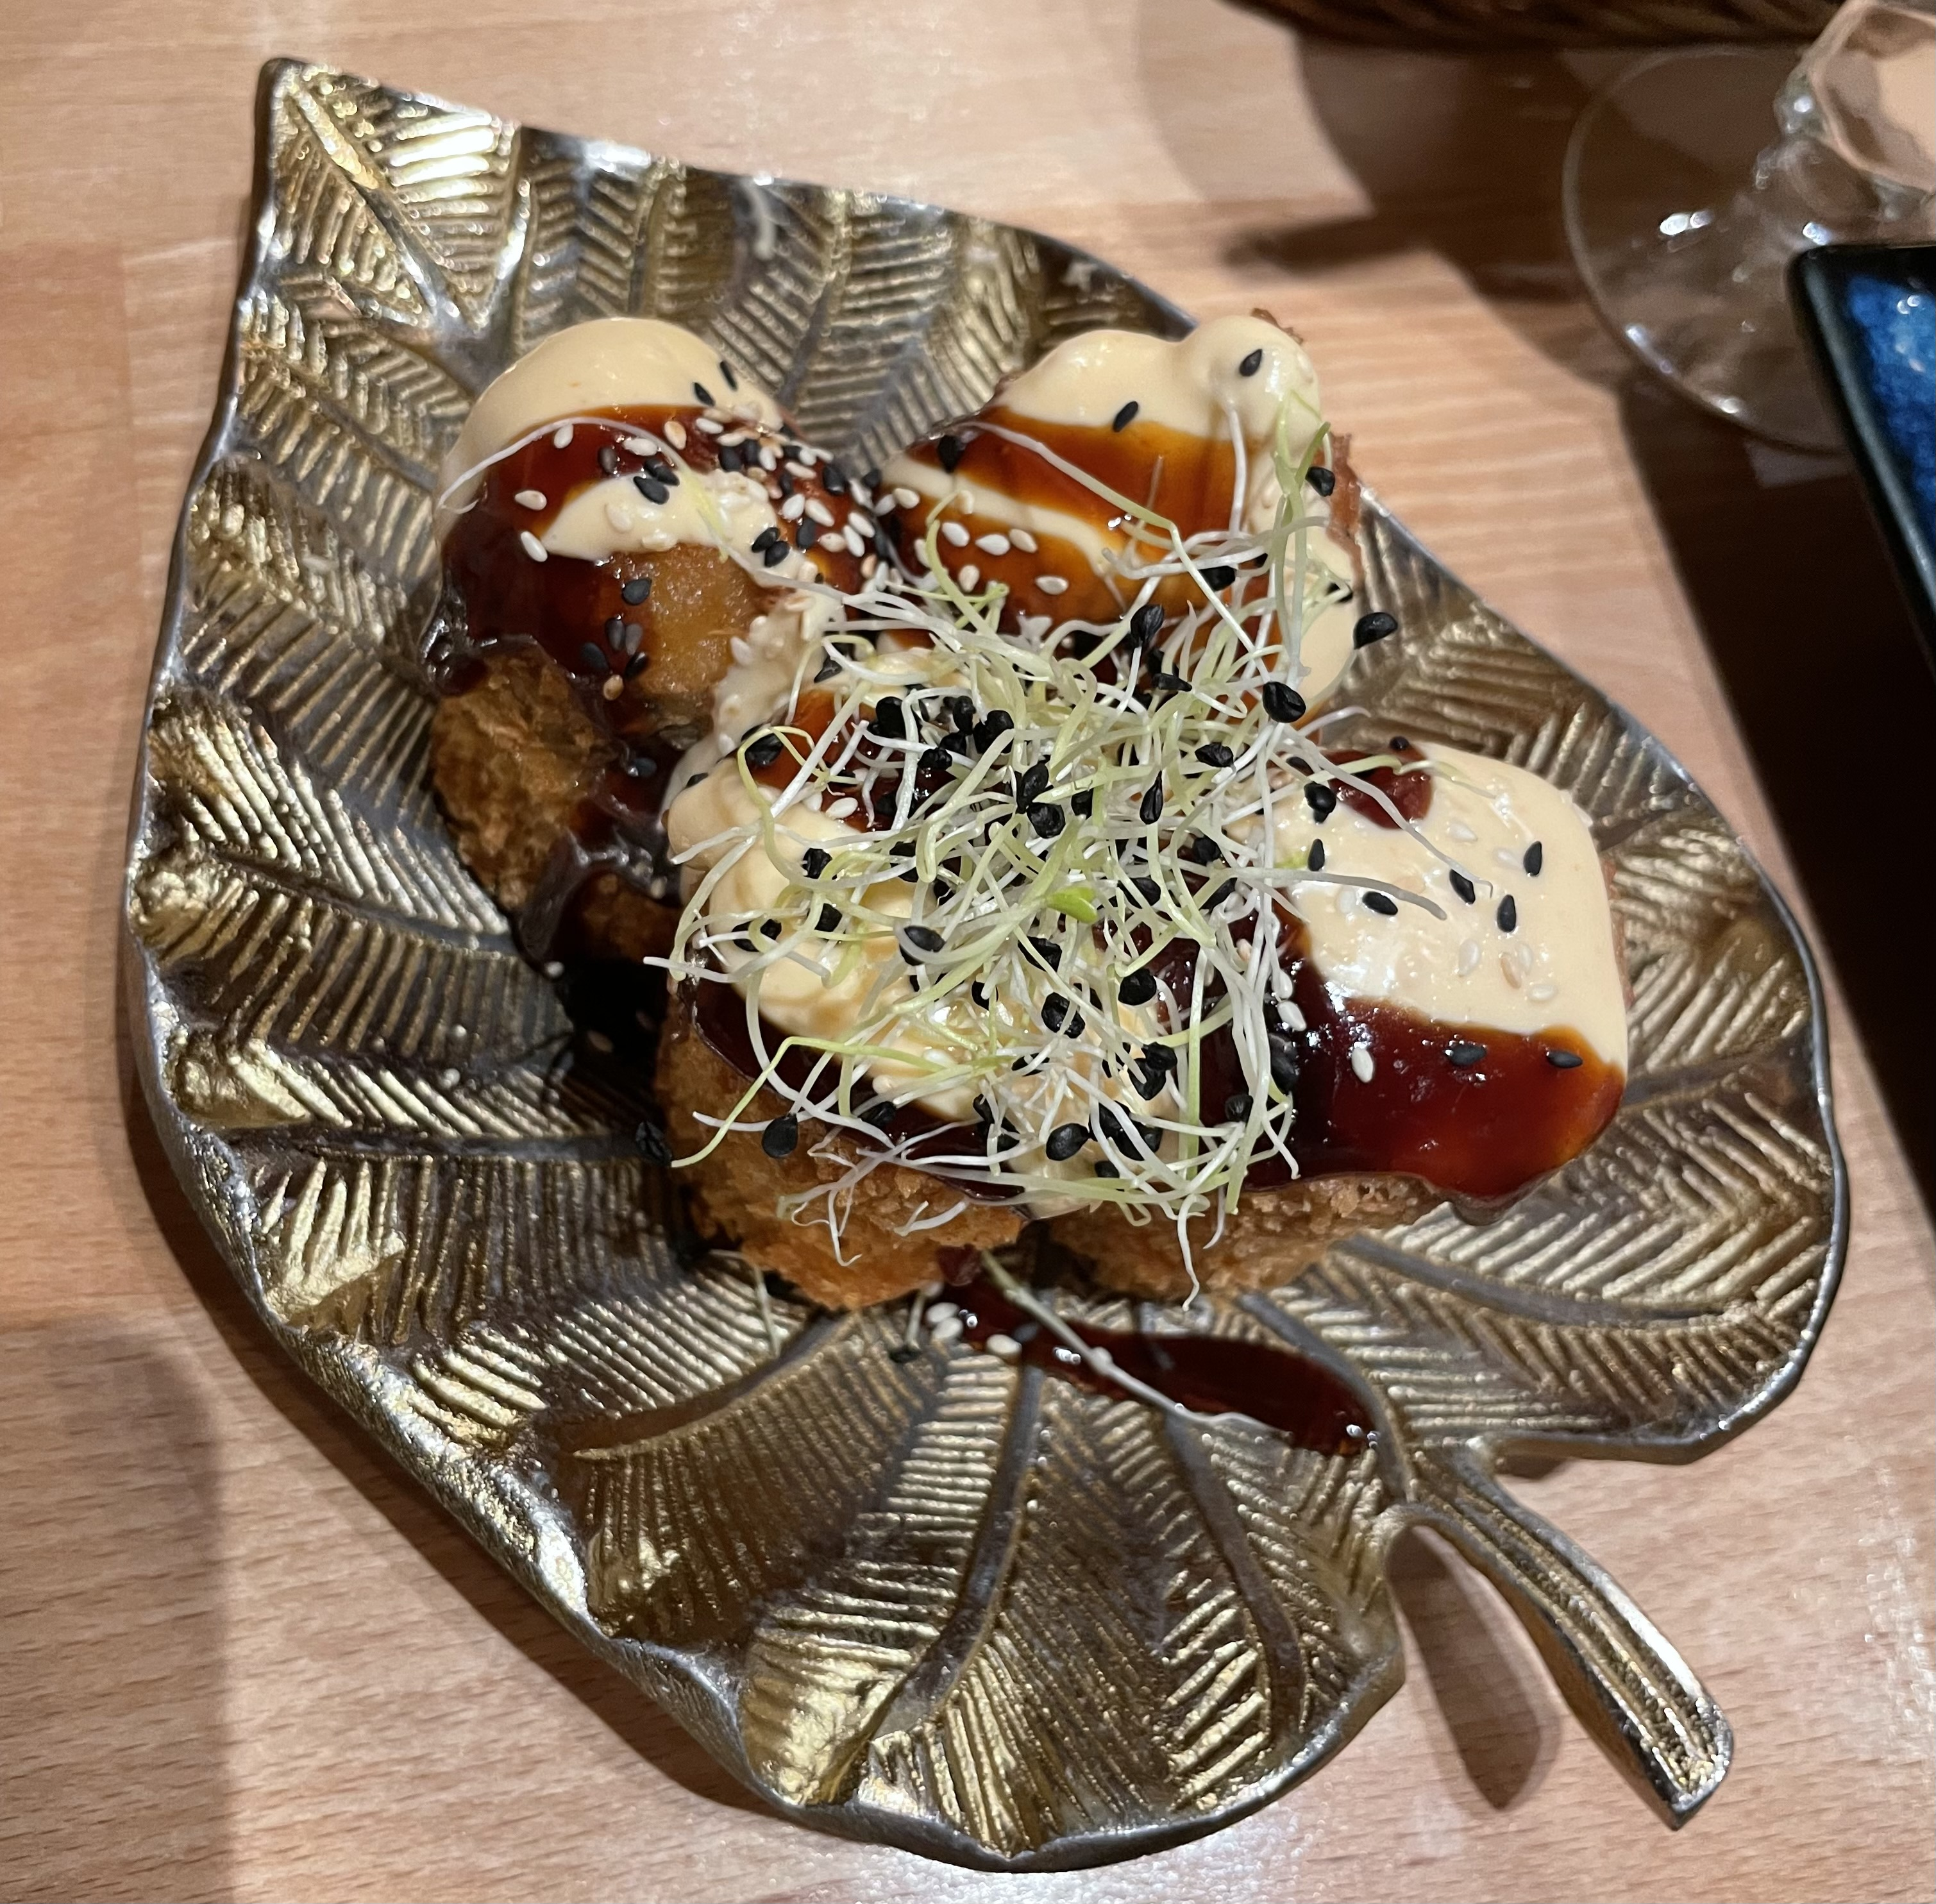
\includegraphics[width=0.9\textwidth]{anlagen/bilder/Bild2.jpg}
        \caption{Bild 2}
        \label{fig:bild2}
    \end{subfigure}
    \caption{Bildunterschrift}
    \label{fig:bilder}
\end{lstlisting}

Im folgenden wird das Ergebnis der obigen Codezeilen dargestellt:

\begin{figure}[H]
    \centering
    \begin{subfigure}{0.45\textwidth}
        \centering
        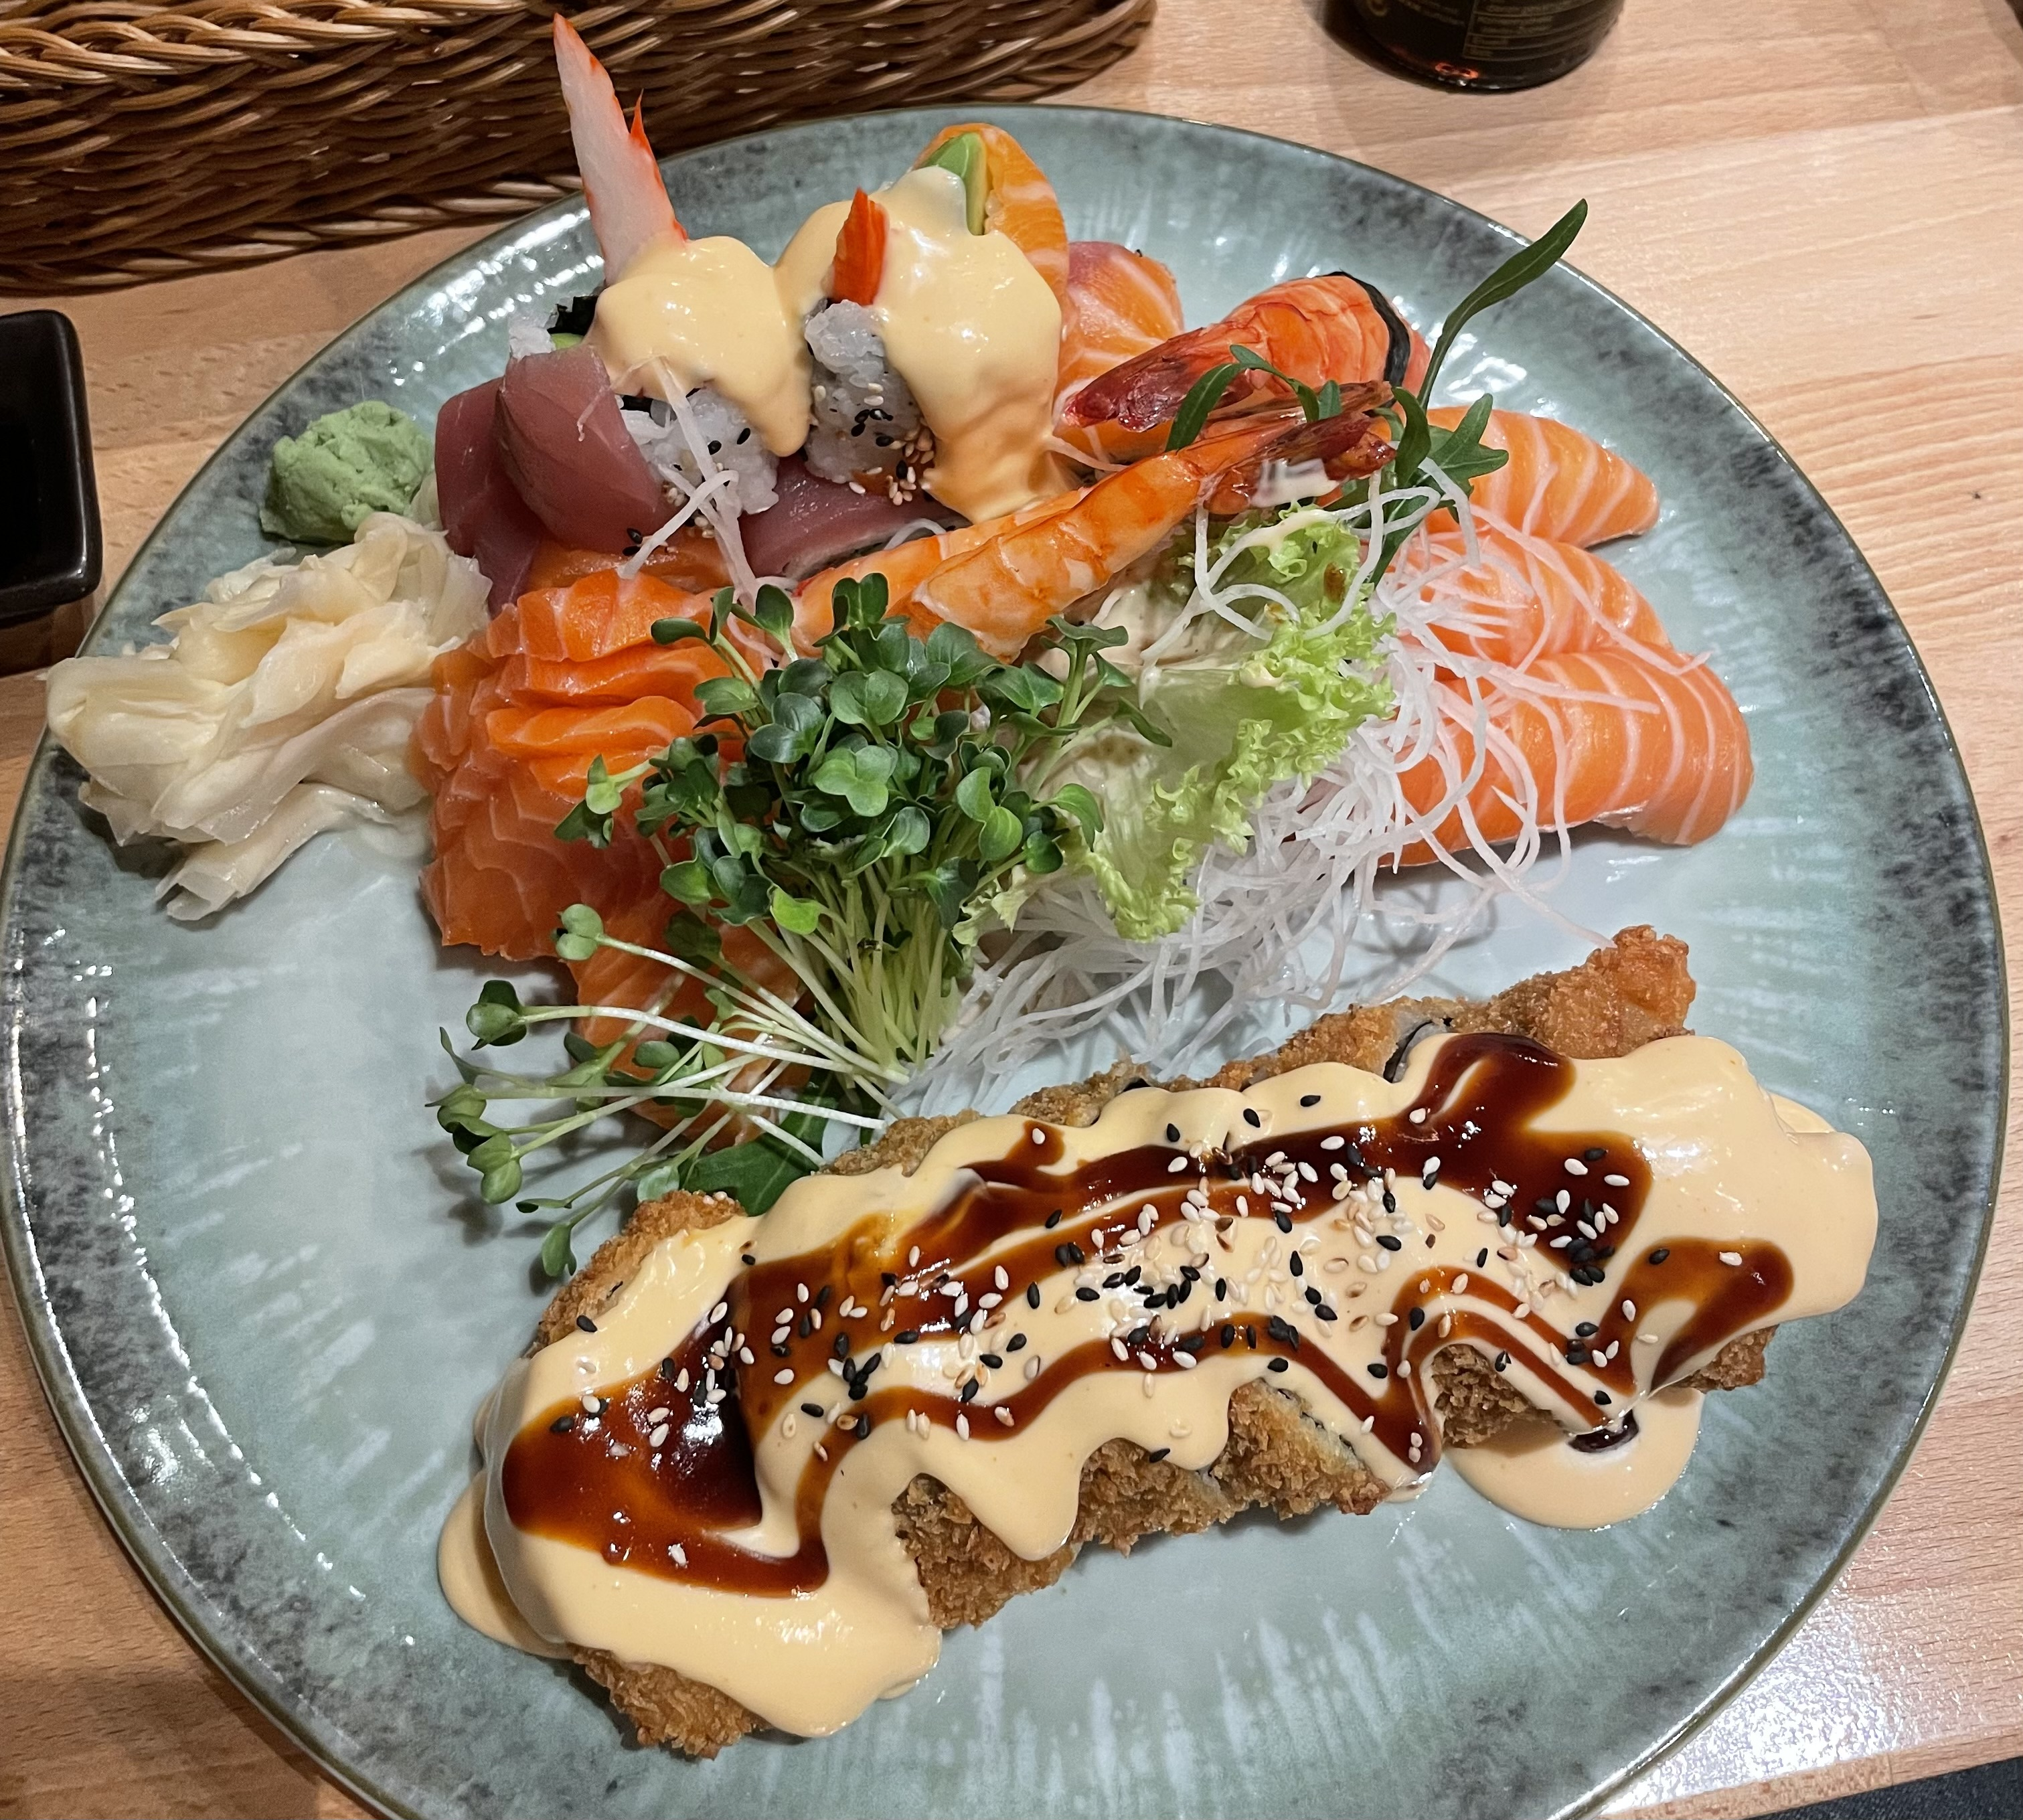
\includegraphics[width=0.9\textwidth]{anlagen/bilder/Bild1.jpg}
        \caption{Bild 1}
        \label{fig:bild1}
    \end{subfigure}
    \hfill
    \begin{subfigure}{0.45\textwidth}
        \centering
        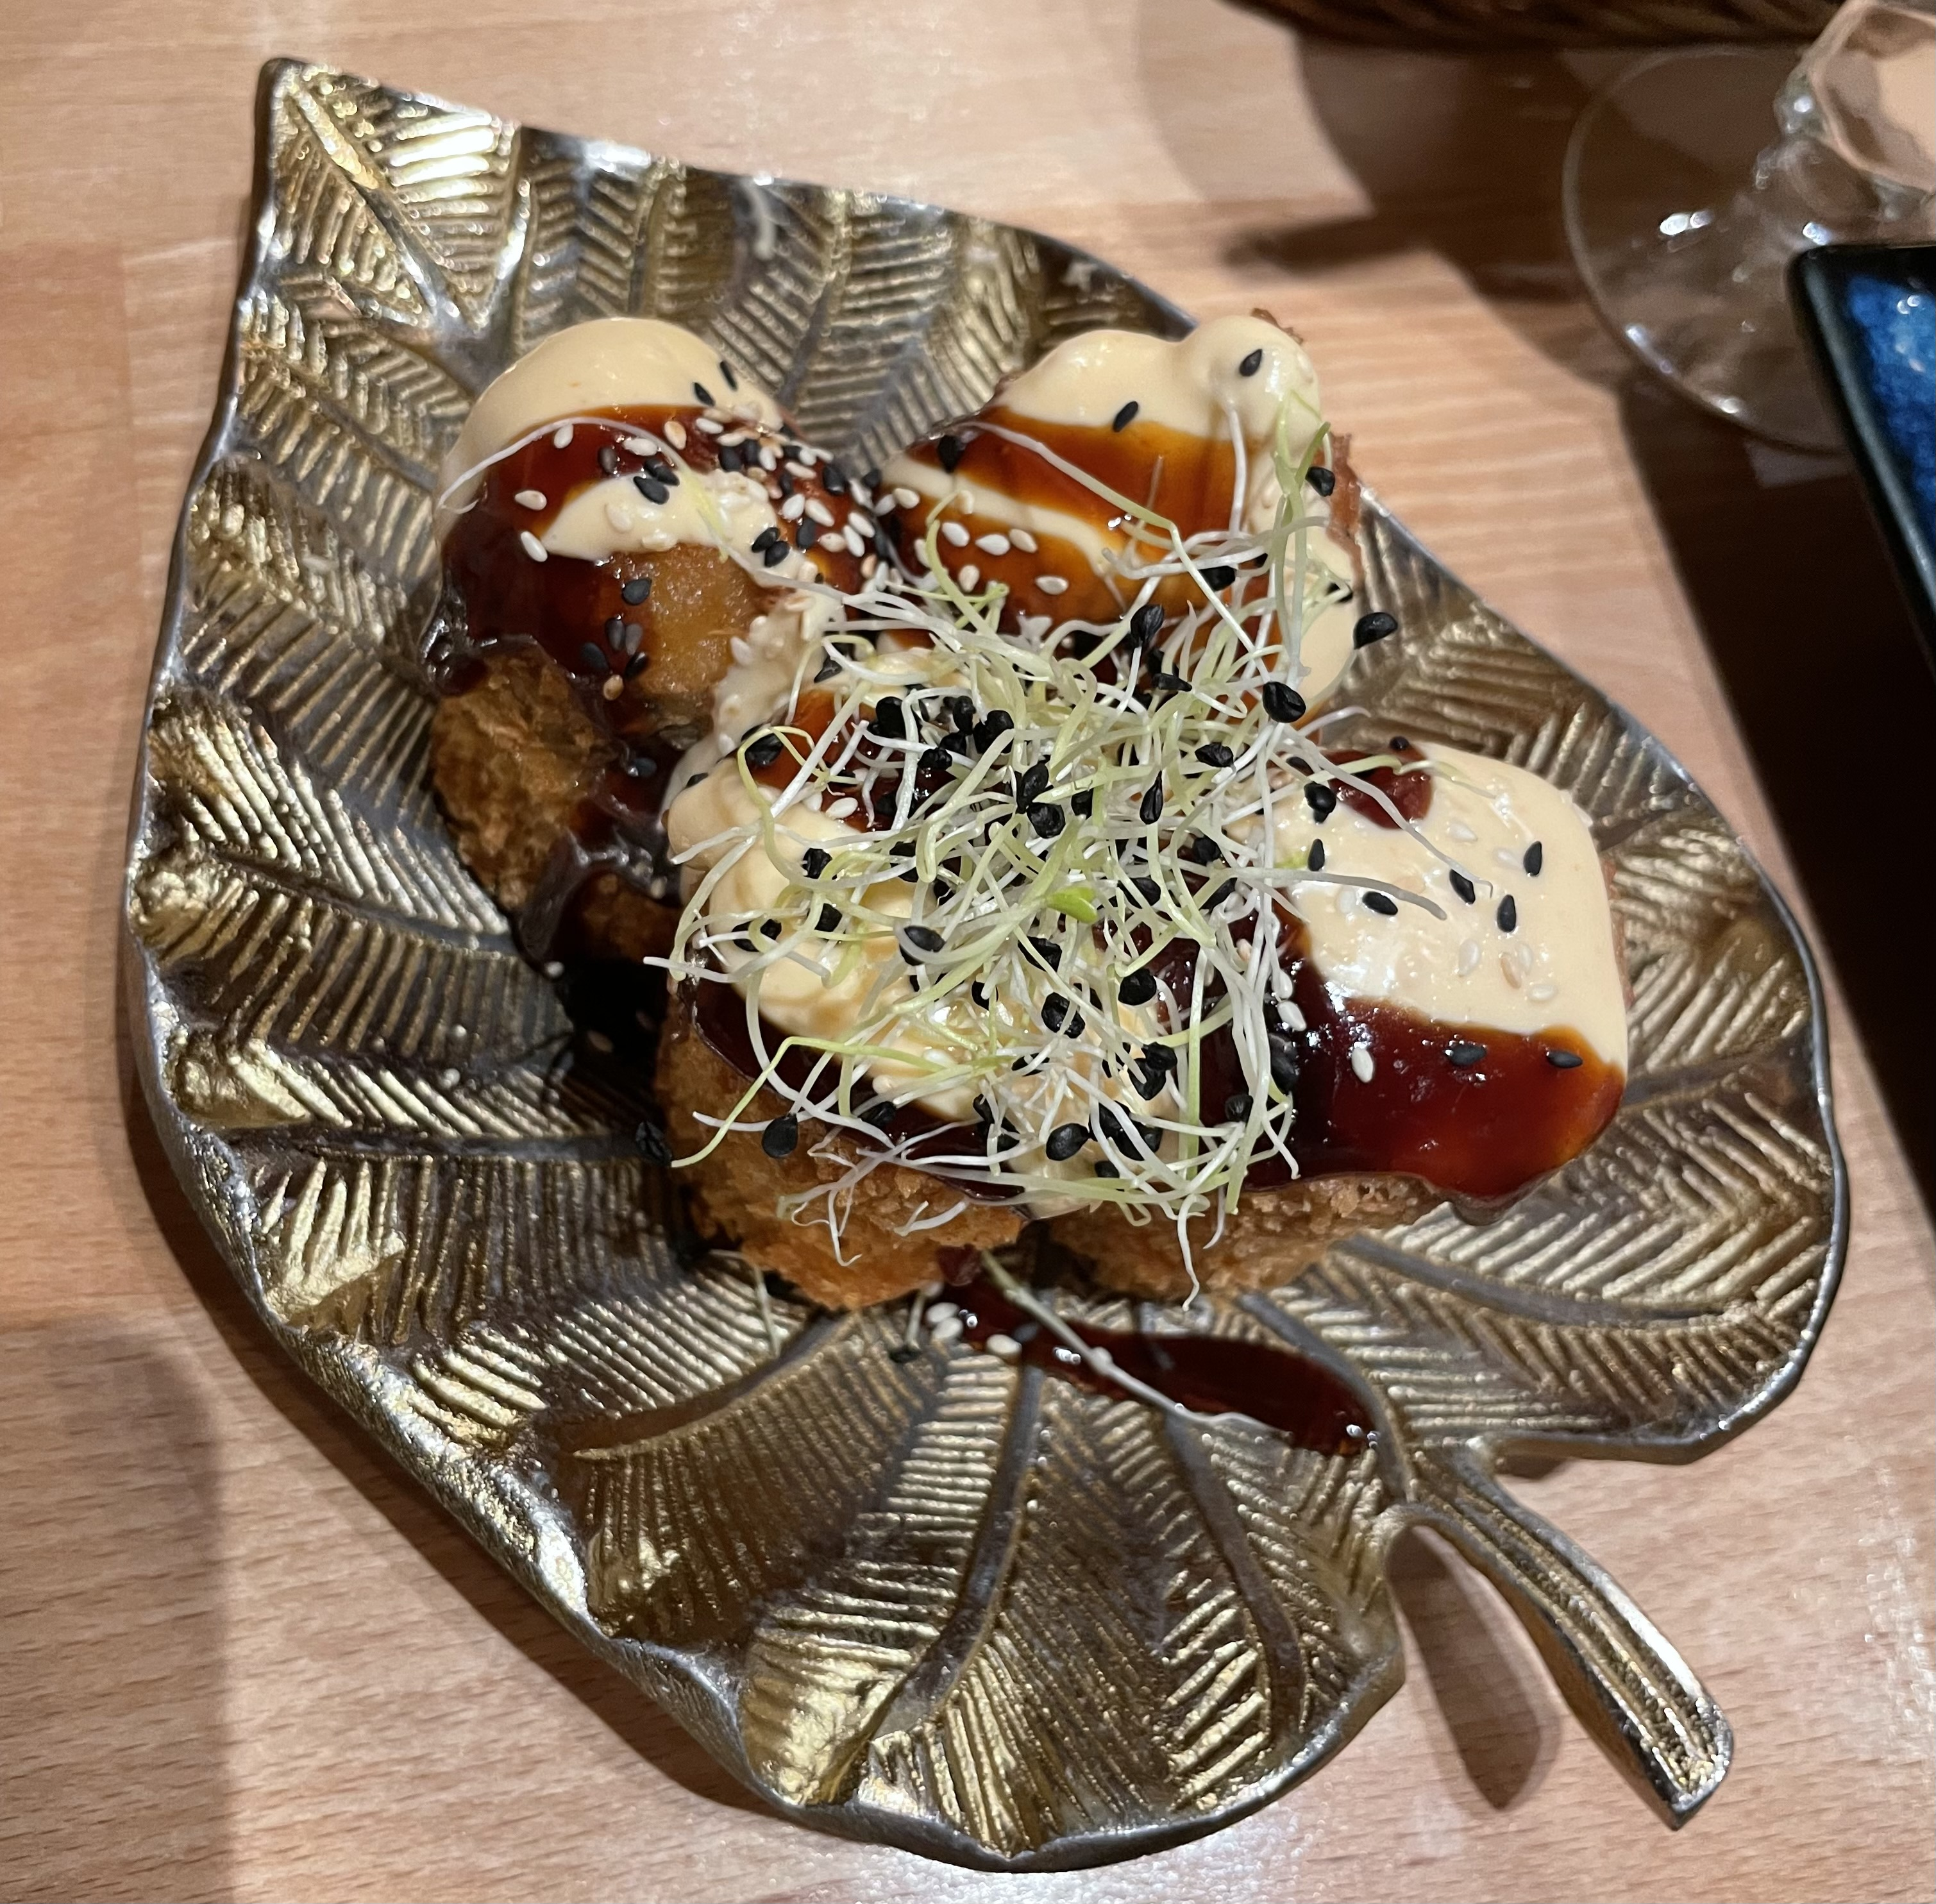
\includegraphics[width=0.9\textwidth]{anlagen/bilder/Bild2.jpg}
        \caption{Bild 2}
        \label{fig:bild2}
    \end{subfigure}
    \caption{Bildunterschrift}
    \label{fig:bilder}
\end{figure}

Besonders praktisch ist die Verwendung der \textbf{\texttt{subfigure}}-Umgebung, um die Bilder mit Untertiteln und Labeln zu versehen, auf die im Text referenziert werden kann (\autoref{fig:bild1}, \autoref{fig:bild2}) und \autoref{fig:bilder}.
In der \textbf{\texttt{subfigure}}-Umgebung können durch geschicktes Aneinanderreihen auch mehr als zwei Bilder nebeneinander (oder untereinander) dargestellt werden.


\subsection{Tabellen}
In \LaTeX{} gibt es mehrere Möglichkeiten, Tabellen zu erstellen. Im Folgenden werden die wichtigsten Möglichkeiten und Optionen vorgestellt.

\subsubsection{Einfache Tabelle}
Eine einfache Tabelle kann mit der \textbf{\texttt{tabular}}-Umgebung erstellt werden. Die Spalten werden durch \textbf{\texttt{\&}} und die Zeilen durch \textbf{\texttt{\textbackslash\textbackslash}} getrennt. Häufig wird die \textbf{\texttt{tabular}}-Umgebung innerhalb einer \textbf{\texttt{table}}-Umgebung verwendet, um die Tabelle zu positionieren, zu beschriften und zu referenzieren (siehe auch: \nameref{sec:querverweise}).

Die \textbf{\texttt{table}}-Umgebung kann mit einer Option \textbf{\texttt{[...]}} versehen werden, um die Positionierung zu steuern (siehe auch: \autoref{tab:figure_options}).

Darüber hinaus können die Spalten mit \textbf{\texttt{l}}, \textbf{\texttt{r}} und \textbf{\texttt{c}} für linksbündig, rechtsbündig und zentriert ausgerichtet werden. Mit \textbf{\texttt{\textbackslash hline}} können vertikale Linien und mit \textbf{\texttt{|}} horizontale Linien eingefügt werden.
Mit \textbf{\texttt{\textbackslash cline\{x-y\}}} können horizontale Linien von Spalte x bis y gezogen werden.

In dem folgenden Beispiel werden zudem die Möglichkeiten doppelter horizontaler Linien (\textbf{\texttt{\textbackslash hline \textbackslash hline}}) und doppelter vertikaler Linien (\textbf{\texttt{||}}) visualisiert.

\begin{minipage}{0.5\textwidth}
    \begin{lstlisting}[language={[LaTeX]TeX}]
\begin{table}[H]
    \centering
    \begin{tabular}{|l||r|c|}
        \hline
        name & age & size \\
        \hline \hline
        Max  & 25    & 1,80m \\
        \hline
        Anna & 22    & 1,65m \\
        \cline{2-2}
        Gustav & 30    & 1,75m \\
        \hline
    \end{tabular}
    \caption{Einfache Tabelle}
    \label{tab:einfache_tabelle}
\end{table}
\end{lstlisting}
\end{minipage}
\hfill
\begin{minipage}{0.5\textwidth}
    \begin{table}[H]
        \centering
        \begin{tabular}{|l||r|c|}
            \hline
            name   & age & size  \\
            \hline \hline
            Max    & 25  & 1,80m \\
            \hline
            Anna   & 22  & 1,65m \\
            \cline{2-2}
            Gustav & 30  & 1,75m \\
            \hline
        \end{tabular}
        \caption{Einfache Tabelle}
        \label{tab:einfache_tabelle}
    \end{table}
\end{minipage}

Mit dem Paket \textbf{\texttt{hhline}} können Linien selektiv gezeichnet werden. Dies kann mit dem Befehl \textbf{\texttt{\textbackslash hhline\{...\}}} erreicht werden.
Die Optionen sind \textbf{\texttt{|}}, \textbf{\texttt{-}}, \textbf{\texttt{=}} und \textbf{\texttt{\textasciitilde}} für vertikale, horizontale, doppelte horizontale und keine Linien.

\begin{minipage}{0.5\textwidth}
    \begin{lstlisting}[language={[LaTeX]TeX}]
\begin{table}[H]
    \centering
    \begin{tabular}{|c|c|c|}
        \hline
        A & B & C \\
        \hhline{|=|-|=|} 
        1 & 2 & 3 \\
        \hhline{|~|-|~|} 
        4 & 5 & 6 \\
        \hhline{|=|=|=|} 
    \end{tabular}
    \caption{Tabelle mit hhline}
    \label{tab:hhline_tabelle}
\end{table}
\end{lstlisting}
\end{minipage}
\hfill
\begin{minipage}{0.5\textwidth}
    \begin{table}[H]
        \centering
        \begin{tabular}{|c|c|c|}
            \hline
            A & B & C \\
            \hhline{|=|-|=|}
            1 & 2 & 3 \\
            \hhline{|~|-|~|}
            4 & 5 & 6 \\
            \hhline{|=|=|=|}
        \end{tabular}
        \caption{Tabelle mit hhline}
        \label{tab:hhline_tabelle}
    \end{table}
\end{minipage}

\subsubsection{Formatierte Tabellen}
Tabellen können mit dem Paktet \textbf{\texttt{array}} formatiert werden.
Formatierungsoptionen können mit dem Befehl \textbf{\texttt{\textbackslash begin\{tabular\}\{...\}}} angegeben werden.

Möglichkeiten sind unter anderem:

\begin{table}[h]
    \centering
    \renewcommand{\arraystretch}{1.3} % Erhöhte Zeilenhöhe für bessere Lesbarkeit
    \setlength{\tabcolsep}{8pt} % Abstände zwischen Spalten setzen
    \begin{tabular}{l|l}
        \toprule
        \textbf{Wirkung}                       & \textbf{Befehl}                                                      \\
        \midrule
        Schriftgröße der Spalte                & >\{\textbackslash small\}c                                           \\
        Fettgedruckte Spalte                   & >\{\textbackslash bfseries\}c                                        \\
        Kursiv formatierte Spalte              & >\{\textbackslash itshape\}c                                         \\
        Farbige Spalte (farbe!deckkraft in \%) & >\{\textbackslash columncolor\{gray!20\}\}c                          \\
        Mathematische Spalte                   & >\{\$\}c<\{\$\}                                                      \\
        \midrule
        Mehrzeilige Spalte (Mitte)             & m\{3cm\}                                                             \\
        Mehrzeilige Spalte (Unten)             & p\{3cm\}                                                             \\
        Mehrzeilige Spalte (Oben)              & b\{3cm\}                                                             \\
        Mehrzeilige Spalte (linksbündig)       & >\{\textbackslash raggedright\textbackslash arraybackslash\}m\{4cm\} \\
        Mehrzeilige Spalte (zentriert)         & >\{\textbackslash centering\textbackslash arraybackslash\}m\{4cm\}   \\
        Mehrzeilige Spalte (rechtsbündig)      & >\{\textbackslash raggedleft\textbackslash arraybackslash\}m\{4cm\}  \\
        \bottomrule
    \end{tabular}
    \caption{Übersicht der array-Formatierungsoptionen}
    \label{tab:array_formatierungen}
\end{table}

Der Befehl \textbf{\texttt{>\{...\}}} sorgt dafür, dass die Formatierung auf die gesamte Spalte angewendet wird.

Es folgt ein Beispiel, dass die verschiedenen Formatierungsmöglichkeiten fette und kursive Schrift, farbige Hintergründe und mathematische Spalten in einer Tabelle darstellt:

\begin{lstlisting}[language={[LaTeX]TeX}, basicstyle=\footnotesize]
\begin{table}[H]
    \centering
    \begin{tabular}{|>{\bfseries}c|>{\itshape}r|>{\columncolor{blue!10}}c|>{$}c<{$}|}
        \hline
        Fett & Kursiv & Farbiger Hintergrund & Mathematische \: Spalte                \\
        \hline
        name & age    & size                 & E = mc^2                               \\
        \hline
        Max  & 25     & 1.80m                & a^2 + b^2 = c^2                        \\
        \hline
        Lisa & 30     & 1.75m                & x = \frac{-b \pm \sqrt{b^2 - 4ac}}{2a} \\
        \hline
    \end{tabular}
    \caption{Fett, Kursiv, Farbiger Hintergrund und Mathematisch}
    \label{tab:formatierte_tabelle}
\end{table}
\end{lstlisting}

\begin{table}[H]
    \centering
    \begin{tabular}{|>{\bfseries}c|>{\itshape}r|>{\columncolor{blue!10}}c|>{$}c<{$}|}
        \hline
        Fett & Kursiv & Farbiger Hintergrund & Mathematische \: Spalte                \\
        \hline
        name & age    & size                 & E = mc^2                               \\
        \hline
        Max  & 25     & 1.80m                & a^2 + b^2 = c^2                        \\
        \hline
        Lisa & 30     & 1.75m                & x = \frac{-b \pm \sqrt{b^2 - 4ac}}{2a} \\
        \hline
    \end{tabular}
    \caption{Fett, Kursiv, Farbiger Hintergrund und Mathematisch}
    \label{tab:formatierte_tabelle}
\end{table}

\subsubsection{Spalten mit Zeilenumbruch}
Es folgt ein Beispiel, dass die verschiedenen Möglichkeiten für Spalten mit Zeilenumbruch aus \autoref{tab:array_formatierungen} darstellt:

\begin{lstlisting}[language={[LaTeX]TeX}, basicstyle=\footnotesize]
\begin{table}[H]
    \centering
    \begin{tabular}{|>{\raggedright\arraybackslash}m{5cm}|>{\centering\arraybackslash}p{4cm}|>{\raggedleft\arraybackslash}b{5cm}|}
        \hline
        Mittig und linksbundig  &   Unten und zentriert &   Oben und rechtsbundig   \\
        \hline
        Dies ist ein langer Text, der linksbundig ausgerichtet ist und umgebrochen wird. & Dies ist ein langer Text, der zentriert ist und am unteren Rand der Zelle ausgerichtet ist. & Dies ist ein langer Text, der rechtsbundig ausgerichtet ist und am oberen Rand der Zelle ausgerichtet ist. \\
        \hline
    \end{tabular}
    \caption{Ausrichtung der Spalten}
    \label{tab:ausrichtung_spalten}
\end{table}
\end{lstlisting}

\begin{table}[H]
    \centering
    \begin{tabular}{|>{\raggedright\arraybackslash}m{5cm}|>{\centering\arraybackslash}p{4cm}|>{\raggedleft\arraybackslash}b{5cm}|}
        \hline
        \textbf{Mittig und linksbündig}                                                  & \textbf{Unten und zentriert}                                                                & \textbf{Oben und rechtsbündig}                                                                             \\
        \hline
        Dies ist ein langer Text, der linksbündig ausgerichtet ist und umgebrochen wird. & Dies ist ein langer Text, der zentriert ist und am unteren Rand der Zelle ausgerichtet ist. & Dies ist ein langer Text, der rechtsbündig ausgerichtet ist und am oberen Rand der Zelle ausgerichtet ist. \\
        \hline
    \end{tabular}
    \caption{Ausrichtung der Spalten}
    \label{tab:ausrichtung_spalten}
\end{table}

\subsubsection{Weitere Formatierungsmöglichkeiten}
In Tabellen können weitere Formatierungsmöglichkeiten vorgenommen werden. Dazu gehören unter anderem:

\begin{table}[H]
    \centering
    \renewcommand{\arraystretch}{1.3} % Erhöhte Zeilenhöhe für bessere Lesbarkeit
    \setlength{\tabcolsep}{8pt} % Abstände zwischen Spalten setzen
    \rowcolors{2}{gray!20}{white} % Alternierende Zeilenfarben
    \begin{tabular}{>{\footnotesize}l|l}
        \toprule
        \rowcolor{gray!40} % Kopfzeilenhintergrund
        \textbf{Wirkung}                          & \textbf{Befehl}                                                                                           \\
        \midrule
        Größere Zeilenhöhe setzen (Standard: 1.0) & \textbackslash renewcommand\{\textbackslash arraystretch\}\{...\}                                         \\
        Spaltenabstand erhöhen (Standard: 6pt)    & \textbackslash setlength\{\textbackslash tabcolsep\}\{...pt\}                                             \\
        Alternierende Zeilenfarben                & \scriptsize{\textbackslash rowcolors\{Startzeile\}\{Farbe-ungerade!Deckkraft\}\{Farbe-gerade!Deckkraft\}} \\
        Kopfzeilenhintergrund setzen              & \textbackslash rowcolor\{gray!40\}                                                                        \\
        \bottomrule
    \end{tabular}
    \caption{Weitere Formatierungsmöglichkeiten für Tabellen}
    \label{tab:weitere_formatierungen}
\end{table}

Die folgenden Befehle aus \autoref{tab:weitere_formatierungen} können in der Präambel der \texttt{\textbf{\textbackslash begin\{table\}[H]}} Umgebung definiert werden.

Als Beispiel sollen die Formatierungsmöglichkeiten, die beim Erstellen der \autoref{tab:weitere_formatierungen} verwendet wurden, dargestellt werden.
Der Code für die Präambel sieht wie folgt aus:

\begin{lstlisting}[language={[LaTeX]TeX}, basicstyle=\small]
\begin{table}[H]
    \centering
    \renewcommand{\arraystretch}{1.3} % Erhohte Zeilenhohe fur bessere Lesbarkeit
    \setlength{\tabcolsep}{8pt} % Abstande zwischen Spalten setzen
    \rowcolors{2}{gray!20}{white} % Alternierende Zeilenfarben
    \begin{tabular}{>{\footnotesize}l|l}
        ...
    \end{tabular}
    \caption{Weitere Formatierungsmoglichkeiten fur Tabellen}
    \label{tab:weitere_formatierungen}
\end{table}
\end{lstlisting}

Darüber hinaus können \textbf{eigene Spaltentypen} definiert werden, um die Formatierung von Tabellen zu vereinfachen. Dazu wird der Befehl \textbf{\texttt{\textbackslash newcolumntype\{Spaltentypname\}\{Formatierung\}}} verwendet. In \autoref{tab:array_formatierungen} sind einige Möglichkeiten zur Formatierung von Spalten aufgeführt. Die neu erstellten Spaltentypen können dann in \textbf{\texttt{\textbackslash begin\{tabular\}\{...\}}} verwendet werden.


\subsubsection{Zeilen oder Spalten verbinden}
Zeilen oder Spalten können in Tabellen mit dem Befehl \newline \textbf{\texttt{\textbackslash multirow\{Anzahl-der-Zeilen\}\{Breite\}\{Inhalt\}}} oder \newline \textbf{\texttt{\textbackslash multicolumn\{Anzahl-der-Spalten\}\{|Ausrichtung|\}\{Inhalt\}}} verbunden werden. Es wird das Paket \textbf{\texttt{multirow}} benötigt.

Die Breite von \textbf{\texttt{\textbackslash multirow}} kann entweder in cm oder als \textbf{\texttt{*}} für die automatische Breiteangabe gesetzt werden. Die Ausrichtung von \textbf{\texttt{\textbackslash multicolumn}} kann entweder \textbf{\texttt{l}}, \textbf{\texttt{c}} oder \textbf{\texttt{r}} für linksbündig, zentriert oder rechtsbündig ausgerichtet werden.

Es folgt ein Beispiel, dass das Verbinden von Zeilen und/oder Spalten in einer Tabelle darstellt:

\begin{lstlisting}[language={[LaTeX]TeX}, basicstyle=\scriptsize]
\begin{table}[H]
    \centering
    \renewcommand{\arraystretch}{1.5}
    \begin{tabular}{|c|c|c|}
        \hline
        \textbf{Spalte 1}                        & \textbf{Spalte 2} & \textbf{Spalte 3} \\
        \hline
        \multirow{2}{*}{\textbf{Mehrere Zeilen}} & Wert A            & Wert B            \\
                                                 & Wert C            & Wert D            \\
        \hline
        Wert E                          & \multicolumn{2}{c|}{\textbf{Mehrere Spalten}} \\
        \hline
        Eintrag 1                                & Eintrag 2         & Eintrag 3         \\
        \hline
    \end{tabular}
    \caption{Beispiel Zeilen oder Spalten verbinden}
    \label{tab:example_multirow_multicolumn}
\end{table}
\end{lstlisting}

\begin{table}[H]
    \centering
    \renewcommand{\arraystretch}{1.5}
    \begin{tabular}{|c|c|c|}
        \hline
        \textbf{Spalte 1}                        & \textbf{Spalte 2}                             & \textbf{Spalte 3} \\
        \hline
        \multirow{2}{*}{\textbf{Mehrere Zeilen}} & Wert A                                        & Wert B            \\
                                                 & Wert C                                        & Wert D            \\
        \hline
        Wert E                                   & \multicolumn{2}{c|}{\textbf{Mehrere Spalten}}                     \\
        \hline
        Eintrag 1                                & Eintrag 2                                     & Eintrag 3         \\
        \hline
    \end{tabular}
    \caption{Beispiel Zeilen oder Spalten verbinden}
    \label{tab:example_multirow_multicolumn}
\end{table}


\subsubsection{Einfügen von Bildern in Tabellen}
Bilder können in Tabellen mit dem Befehl \textbf{\texttt{\textbackslash includegraphics[...]\{Pfad/zum/Bild.png\}}} eingefügt werden. Dabei können die gleichen Optionen wie bei der normalen Einbindung von Bildern verwendet werden. Besonders praktisch ist die Option \textbf{\texttt{[width=...\textbackslash linewidth]}} um die Breite des Bildes an die Spaltenbreite anzupassen.

\begin{minipage}{0.62\textwidth}
    \begin{lstlisting}[language={[LaTeX]TeX}, basicstyle=\scriptsize]
\begin{table}[H]
    \centering
    \begin{tabular}{|>{\centering\arraybackslash}m{4cm}|c|}
        \hline
        \textbf{Spalte 1}   &   \textbf{Spalte 2} \\
        \hline
        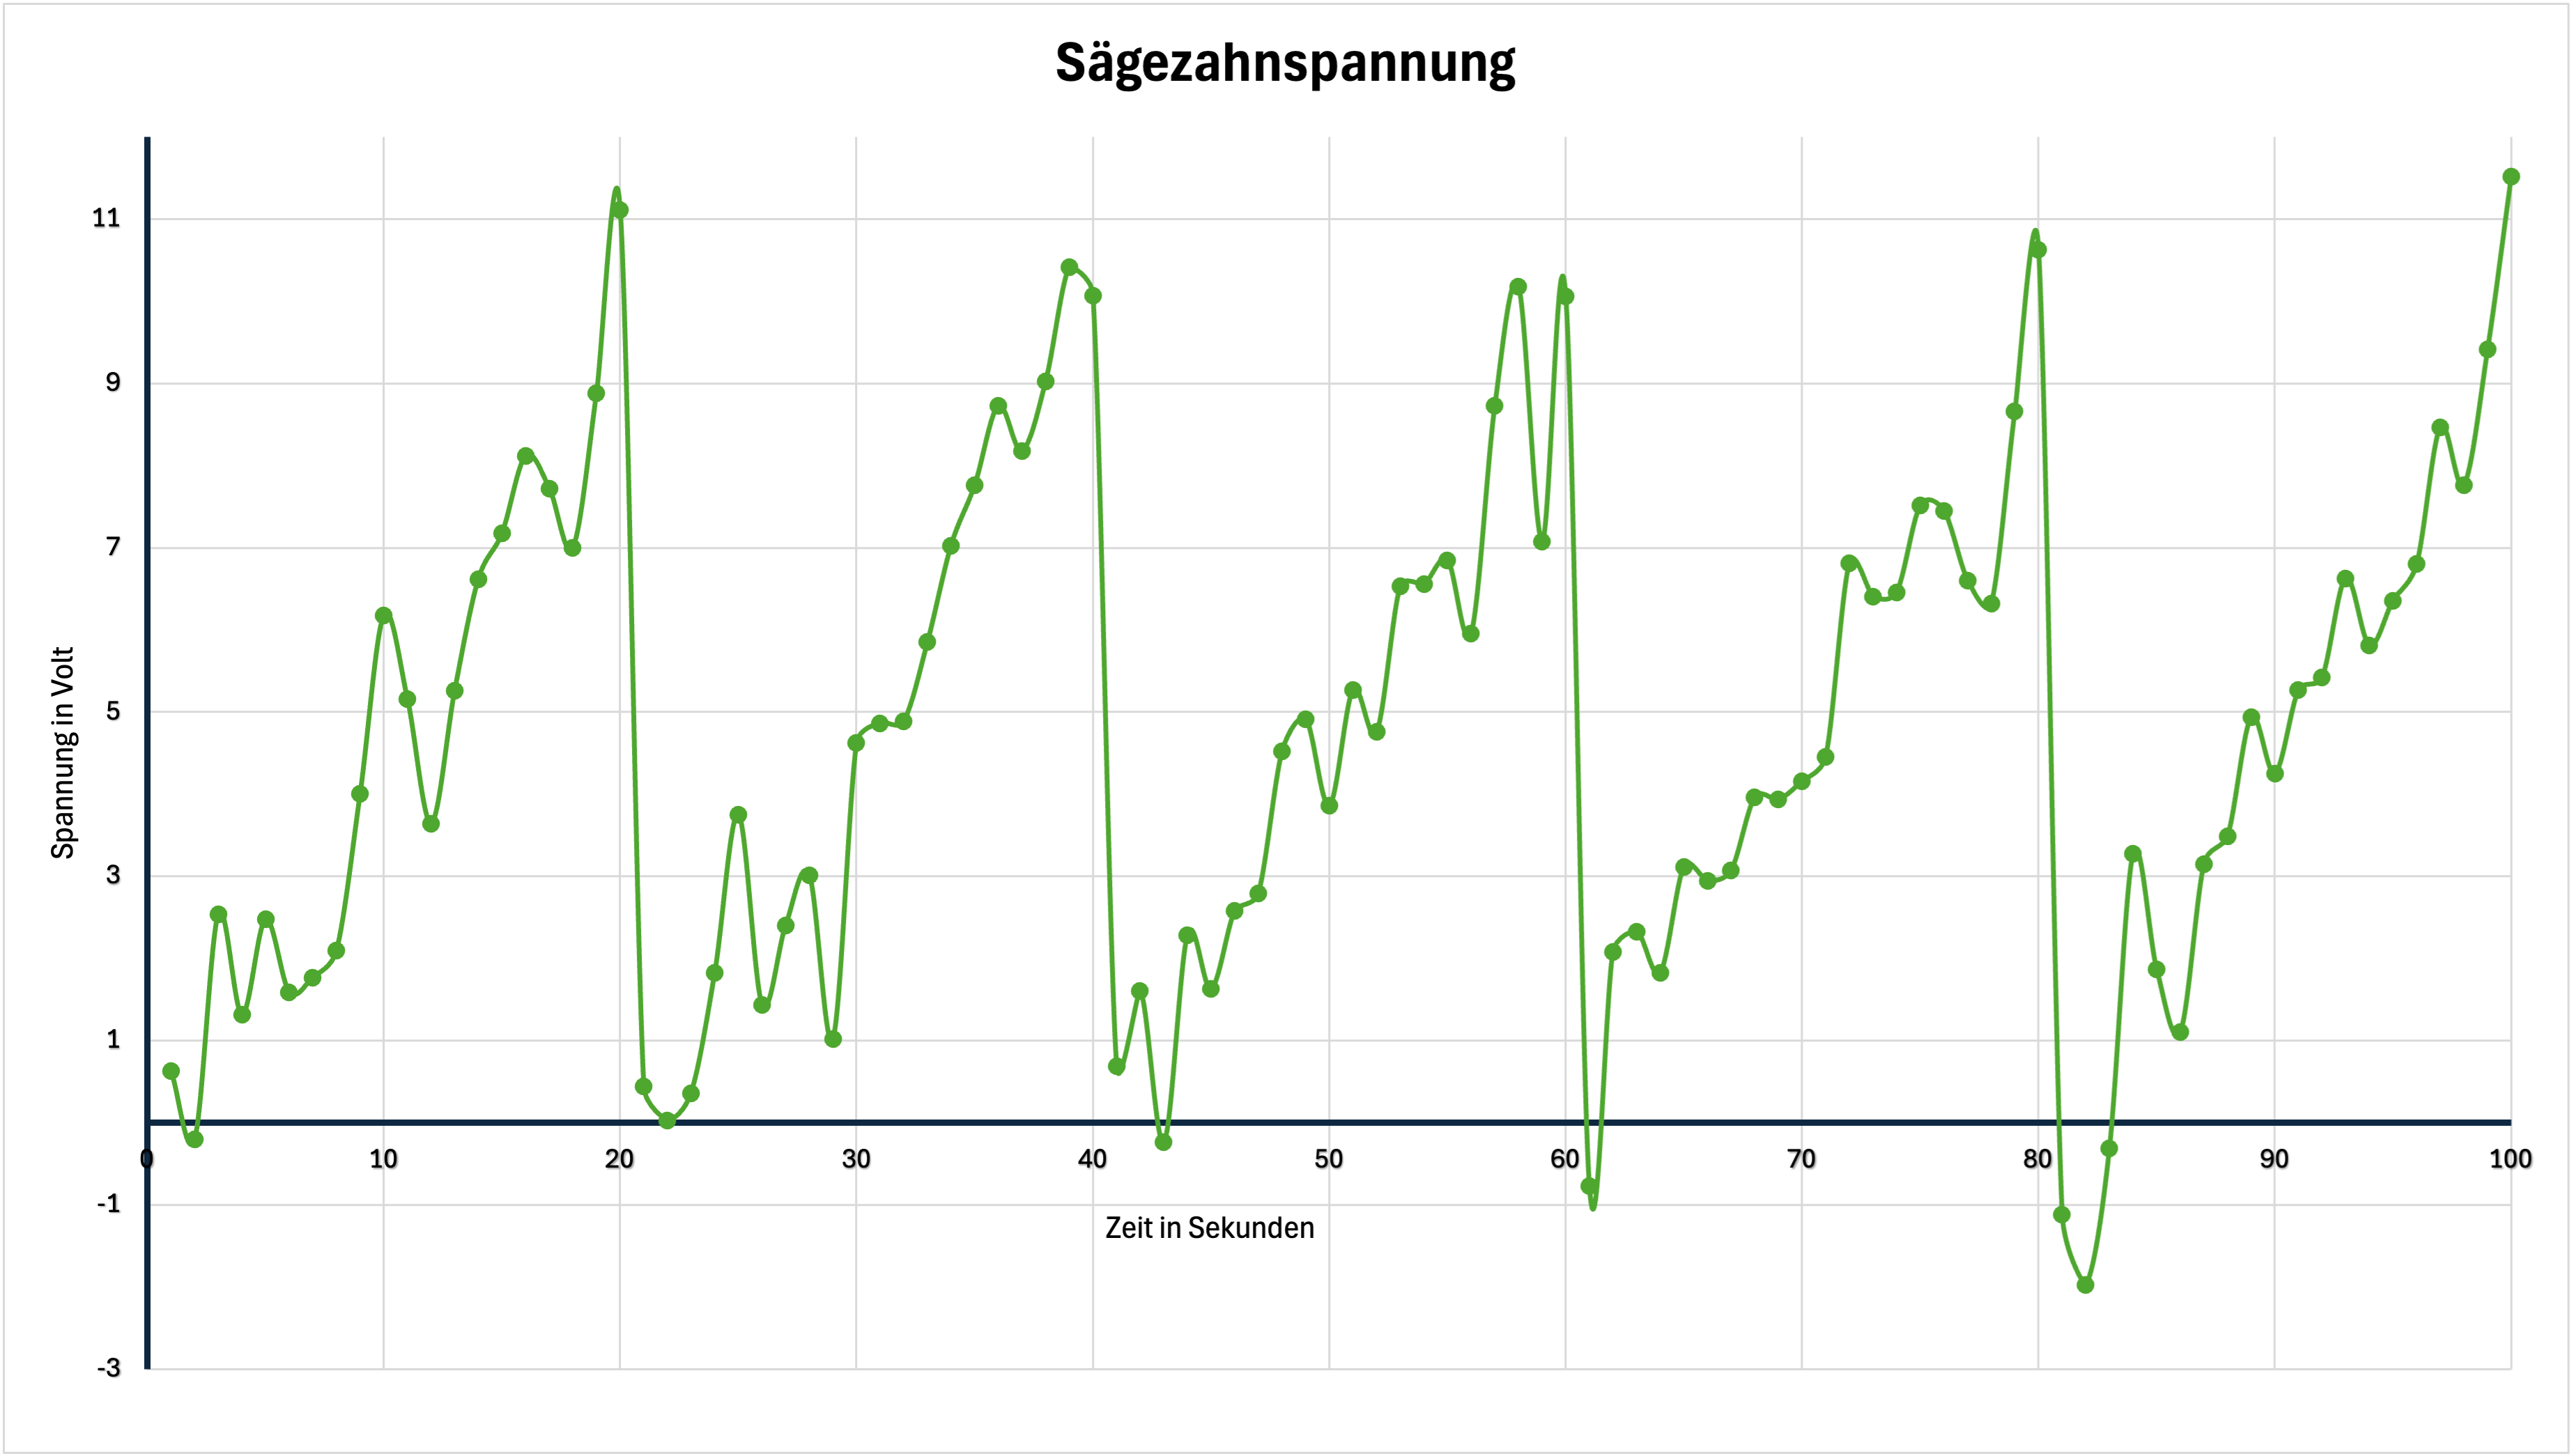
\includegraphics[width=0.8\linewidth]{anlagen/bilder/Graph.png}   &   Text   \\
        \hline
    \end{tabular}
    \caption{Bild in Tabelle}
    \label{tab:bild_in_tabelle}
\end{table}
    \end{lstlisting}
\end{minipage}
\hfill
\begin{minipage}{0.34\textwidth}
    \begin{table}[H]
        \centering
        \begin{tabular}{|>{\centering\arraybackslash}m{3.5cm}|c|}
            \hline
            \textbf{Spalte 1}                                               & \textbf{Spalte 2} \\
            \hline
            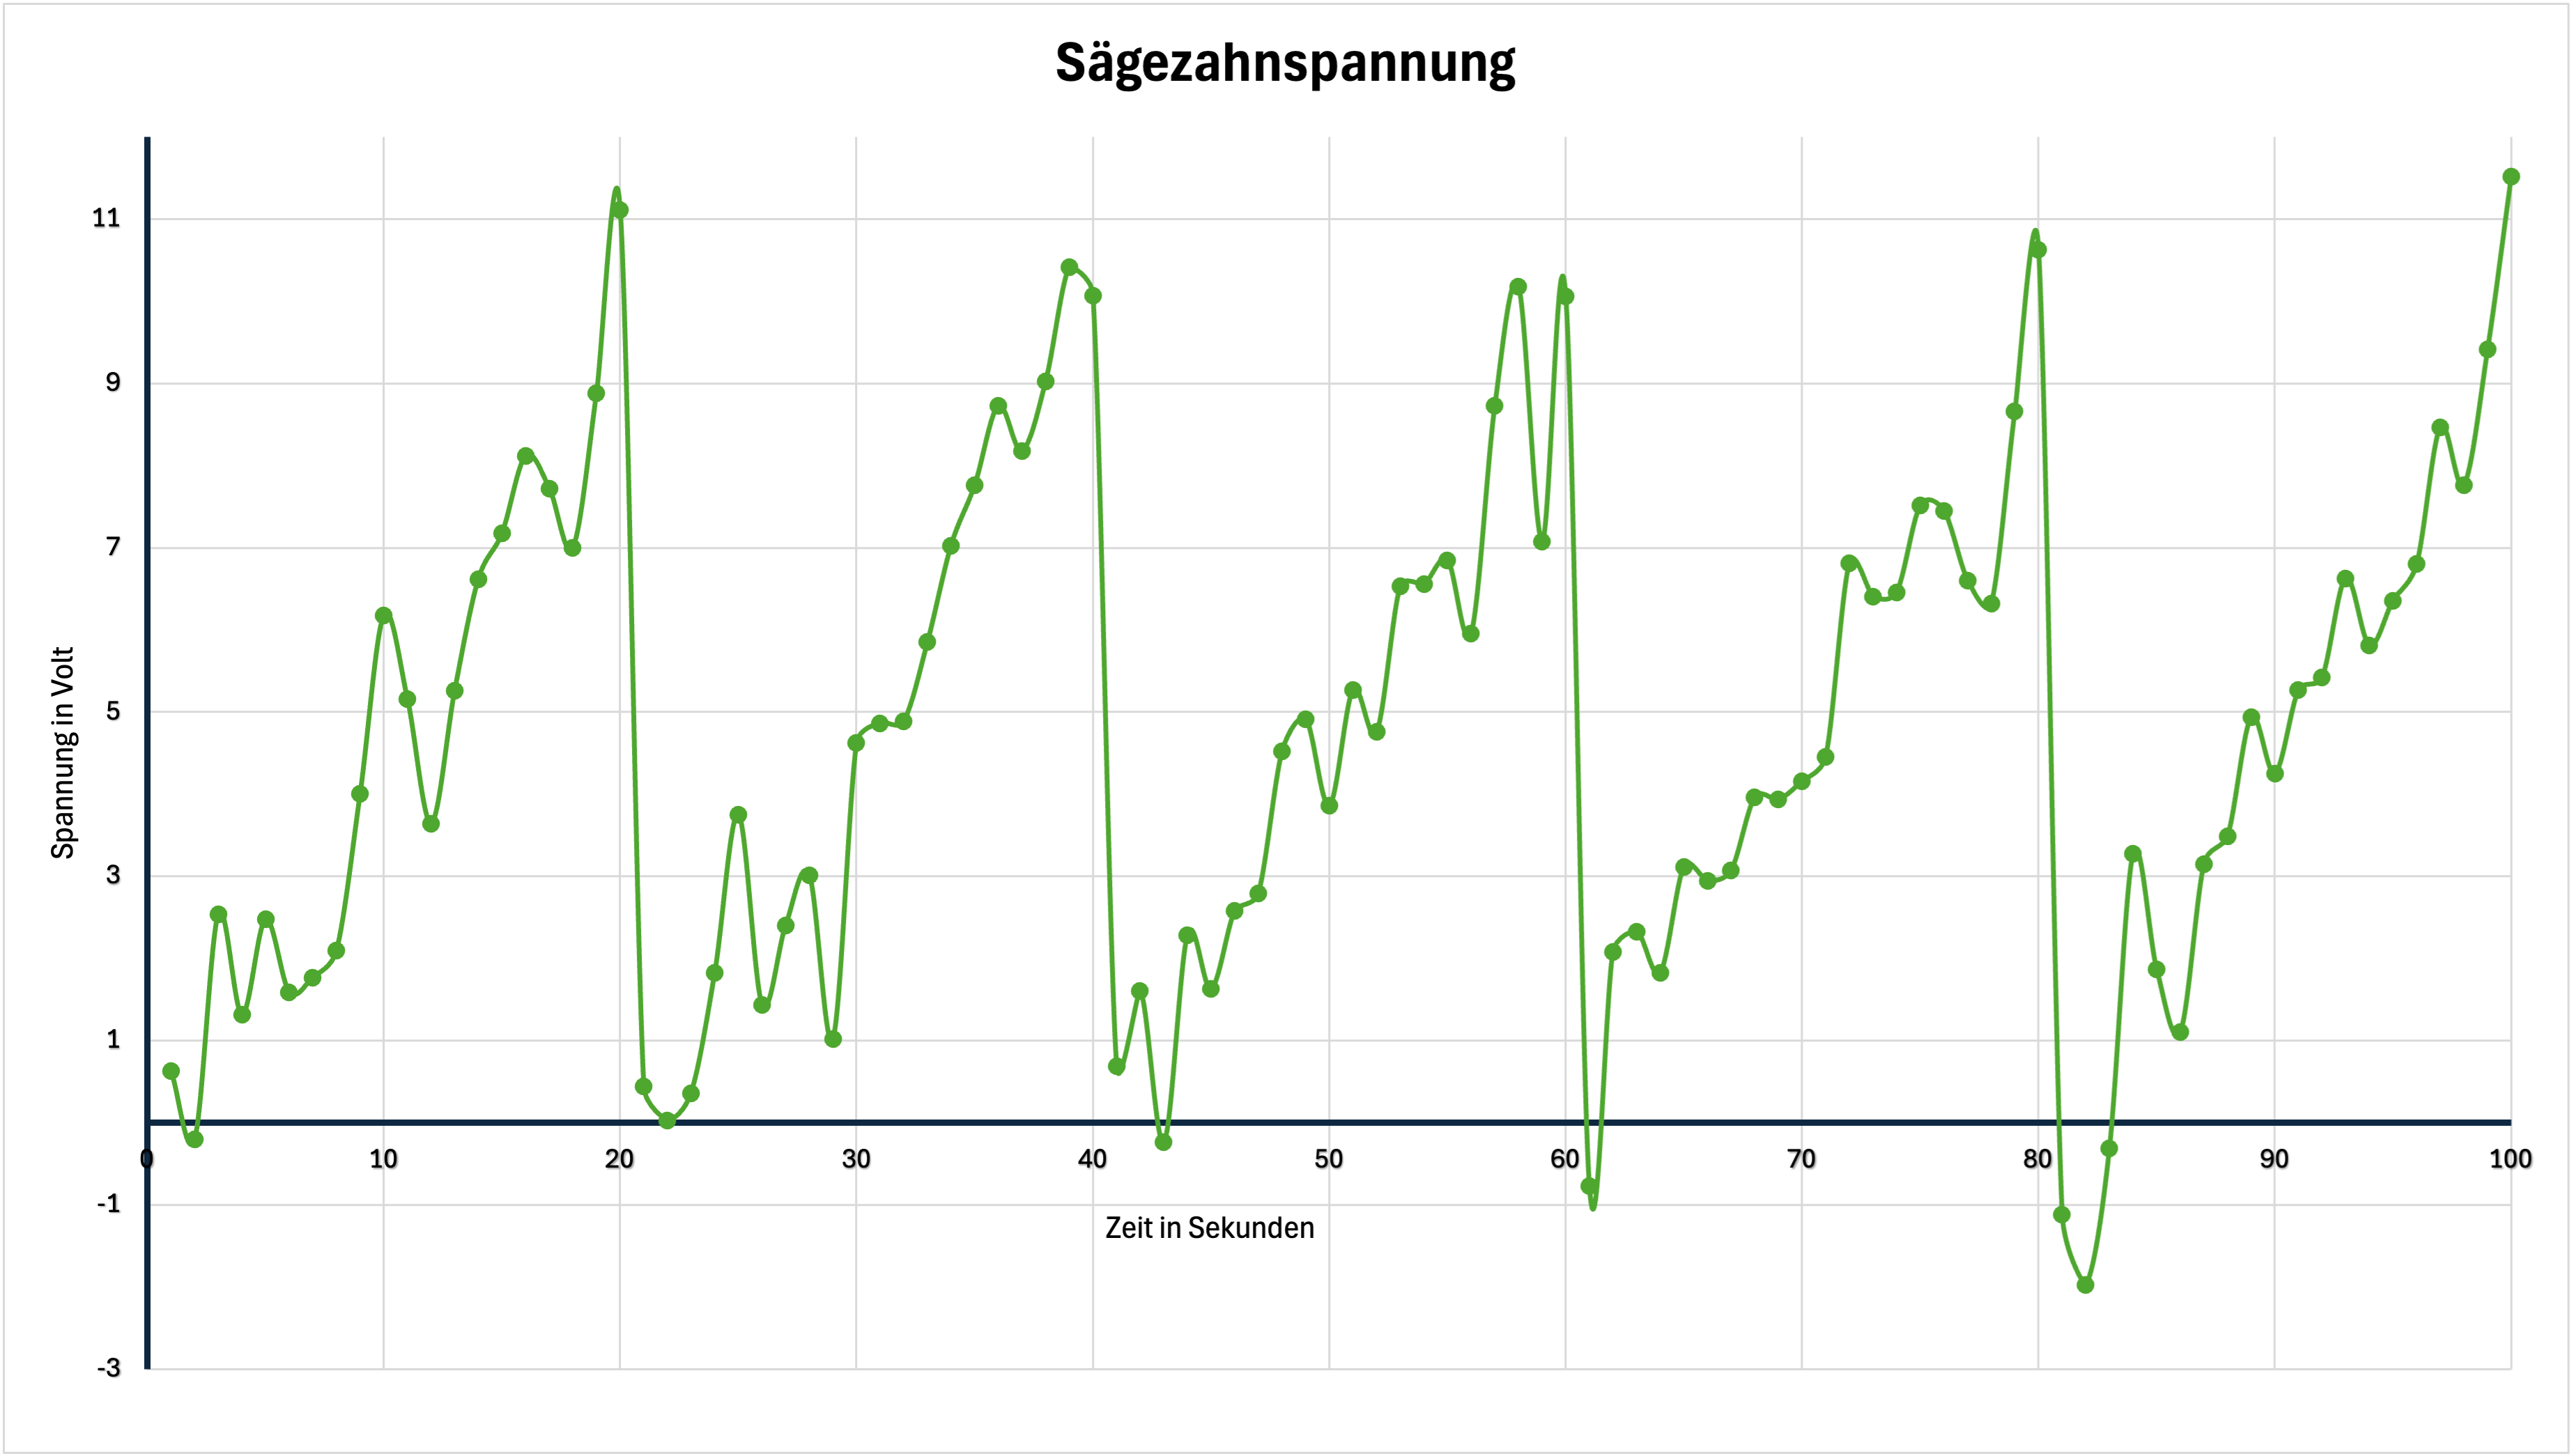
\includegraphics[width=0.8\linewidth]{anlagen/bilder/Graph.png} & Text              \\
            \hline
        \end{tabular}
        \caption{Bild in Tabelle}
        \label{tab:bild_in_tabelle}
    \end{table}
\end{minipage}

\subsubsection{Professionelle Buchtabellen}
Für professionelle Buchtabellen wird das Paket \textbf{\texttt{booktabs}} benötigt. Es bietet die Möglichkeit, Tabellen mit dezenten Linien zu erstellen.

Die Linien können mit \textbf{\texttt{\textbackslash toprule}}, \textbf{\texttt{\textbackslash midrule}} und \textbf{\texttt{\textbackslash bottomrule}} definiert werden. Mit \newline \textbf{\texttt{\textbackslash cmidrule(Optionen)\{Startspalte-Endspalte\}}} kann eine Linie nur für bestimmte Spalten definiert werden. Die Optionen sind  \textbf{\texttt{l}} für eine links, \textbf{\texttt{r}} für eine rechts und \textbf{\texttt{lr}} für eine links und rechts weich abgeschnittene Linie .

\begin{minipage}{0.70\textwidth}
    \begin{lstlisting}[language={[LaTeX]TeX}, basicstyle=\small]
\begin{table}[H]
    \centering
    \begin{tabular}{l|cr}
        \toprule
        \textbf{name} & \textbf{age} & \textbf{size} \\
        \midrule
        Max           & 25           & 1,80m         \\
        \cmidrule(lr){2-3} % Linie nur fur Spalte 2-3
        Anna          & 22           & 1,65m         \\
        \midrule[2pt]
        Gustav        & 30           & 1,75m         \\
        \addlinespace[10pt] % extra Abstand 
        Anna          & 35           & 1,85m         \\
        \bottomrule
    \end{tabular}
    \caption{Buchtabelle}
    \label{tab:booktabs_example}
\end{table}
    \end{lstlisting}
\end{minipage}
\hfill
\begin{minipage}{0.3\textwidth}
    \begin{table}[H]
        \centering
        \begin{tabular}{l|cr}
            \toprule
            \textbf{name} & \textbf{age} & \textbf{size} \\
            \midrule
            Max           & 25           & 1,80m         \\
            \cmidrule(lr){2-3}  % Linie nur für Spalte 2-3
            Anna          & 22           & 1,65m         \\
            \midrule[2pt]
            Gustav        & 30           & 1,75m         \\
            \addlinespace[10pt] % extra Abstand 
            Anna          & 35           & 1,85m         \\
            \bottomrule
        \end{tabular}
        \caption{Buchtabelle}
        \label{tab:booktabs_example}
    \end{table}
\end{minipage}

Die dicke der Linien kann mit \textbf{\texttt{\textbackslash midrule[...pt]}} angepasst werden. Ist ein breiterer Abstand zwischen den Linien gewünscht, kann dies mit \textbf{\texttt{\textbackslash addlinespace[...pt]}} erreicht werden.

\subsubsection{Tabellen über mehrere Seiten}
Tabellen können sich oft über mehrere Seiten erstrecken. Damit ein Seitenumbruch erfolgen kann, wird das Paket \textbf{\texttt{longtable}} benötigt. Seitenumbrüchen können für normale Tabellen und für Buchtabellen ermöglicht werden. Es folgt die Einstellungen für das in \autoref{tab:operatoren} dargestellte Beispiel:

\begin{lstlisting}[language={[LaTeX]TeX}, emph={\endfirsthead,\endhead,\endfoot,\endlastfoot}, emphstyle={\color{red}}]
\begin{longtable}{l l l}
    % Ueberschrift fuer die erste Seite
    \toprule
    \textbf{Operator}  &  \textbf{LaTeX-Code}  &  \textbf{Beispiel}  \\
    \midrule
    \endfirsthead

    % Ueberschrift fuer alle folgenden Seiten
    \toprule
    \textbf{Operator}  &  \textbf{LaTeX-Code}  &  \textbf{Beispiel}  \\
    \midrule
    \endhead

    % Fusszeile fuer jede Seite
    \bottomrule
    \multicolumn{3}{c}{\textit{Fortsetzung auf der naechsten Seite}}
    \endfoot

    % Letzte Fusszeile der Tabelle
    \bottomrule
    \caption{Wichtige Rechenoperatoren und mathematische Symbole}
    \label{tab:operatoren}
    \endlastfoot

    ... 
    \midrule
    ... 

\end{longtable}
\end{lstlisting}

\subsubsection{Tabellen mit farbigen Zellen}
Tabellenzellen können mit dem Paket \textbf{\texttt{xcolor}} farbig gestaltet werden

Der Befehl \textbf{\texttt{\textbackslash cellcolor\{Farbe!Deckkraft\}}} färbt die Zelle ein. Der Befehl \textbf{\texttt{\textbackslash rowcolor\{Farbe!Deckkraft\}}} färbt die gesamte Zeile ein. Soll nur die Schrift farbig sein, kann der Befehl \textbf{\texttt{\textbackslash textcolor\{Farbe\}}} verwendet werden (siehe auch: \ref{sec:schriftfarbe}).

\begin{minipage}{0.69\textwidth}
    \begin{lstlisting}[language={[LaTeX]TeX}, basicstyle=\small]
\begin{table}[H]
    \centering
    \begin{tabular}{|c|c|c|}
        \hline
        \rowcolor{gray!40} % Kopfzeilenhintergrund
        \textbf{Spalte 1} & \textbf{Spalte 2} & \textbf{Spalte 3} \\
        \hline
        \cellcolor{red!25} Wert A & Wert B & Wert C \\
        \hline
        Wert D & \cellcolor{green!25} Wert E & \textcolor{yellow!90}{Wert F} \\
        \hline
    \end{tabular}
    \caption{Tabellen mit farbigen Zellen}
    \label{tab:farbige_zellen}
\end{table}
    \end{lstlisting}
\end{minipage}
\hfill
\begin{minipage}{0.29\textwidth}
    \begin{table}[H]
        \centering
        \begin{tabular}{|c|c|c|}
            \hline
            \rowcolor{gray!40} % Kopfzeilenhintergrund
            \textbf{Spalte 1}         & \textbf{Spalte 2}           & \textbf{Spalte 3}             \\
            \hline
            \cellcolor{red!25} Wert A & Wert B                      & Wert C                        \\
            \hline
            Wert D                    & \cellcolor{green!25} Wert E & \textcolor{yellow!90}{Wert F} \\
            \hline
        \end{tabular}
        \caption{Tabellen mit farbigen Zellen}
        \label{tab:farbige_zellen}
    \end{table}
\end{minipage}


\subsubsection{Hilfreiche Internetseite}
Latex Tabellen können auch mit dem Online-Tool \href{https://tablesgenerator.com/latex_tables}{Tables Generator} erstellt werden. Dieses Tool bietet eine grafische Benutzeroberfläche, um Tabellen zu erstellen und den entsprechenden \LaTeX-Code zu generieren. Die genannte Webseite bietet auch die Möglichkeit, Tabellen aus Excel-Dateien zu importieren und den entsprechenden \LaTeX-Code zu generieren.

Eine weitere Internetseite, die die Konvertierung von Tabellen aus Excel-Dateien in \LaTeX-Code ermöglicht, ist \href{https://www.latex-tables.com}{Latex-Tables}.


\subsection{Mehrspaltige Layouts}

\subsubsection{Minipage}
\label{sec:minipage}
Mit der \textbf{\texttt{minipage}}-Umgebung können mehrspaltige Layouts erstellt werden.
Die grundlegende Syntax ist:
\begin{lstlisting}[language={[LaTeX]TeX}]
\begin{minipage}[Ausrichtung]{Breite}
    Inhalt
\end{minipage}
\end{lstlisting}

Als Ausrichtung können folgende Optionen verwendet werden. Die Verwendung einer Ausrichtung ist allerdings optional (Standard: [c]):

\begin{description}
    \item[c] zentriert
    \item[t] an oberer Kante ausgerichtet
    \item[b] an unterer Kante ausgerichtet
\end{description}

Die Breite kann in cm, mm, pt oder als \texttt{...\textbackslash textwidth} angegeben werden.

Minipages werden in der Regel verwendet um Text und/oder Objekte nebeneinander platzieren zu können.
Allerdings ist zu beachten, dass in einer \textbf{\texttt{minipage}}-Umgebung \textbf{keine Gleitobjekte} wie \texttt{figure} oder \texttt{table} verwendet werden können. Daher müssen Captions mit \textbf{\texttt{\textbackslash captionof\{...\}}} erstellt werden.

Eine Ausnahme bilden Gleitobjekte in Verbindung mit der \textbf{\texttt{[H]}}-Ausrichtung.

\begin{lstlisting}[language={[LaTeX]TeX}, basicstyle=\small]
\begin{minipage}[c]{0.45\textwidth}
    \begin{table}[H]
        \centering
        \begin{tabular}{|c|c|}
            \hline
            \textbf{Wert 1} & \textbf{Wert 2} \\
            \hline
            1               & 2               \\
            3               & 4               \\
            \hline
        \end{tabular}
        \caption{Beispiel Tabelle}
        \label{tab:beispiel_tabelle}
    \end{table}
    Dies ist eine Tabelle, in der einige Daten aufgefuhrt sind.
\end{minipage}
\hfill
\begin{minipage}[c]{0.45\textwidth}
    Es folgt ein Bild, welches eine verrauschte Sagezahnspannung darstellt.
    \begin{figure}[H]
        \centering
        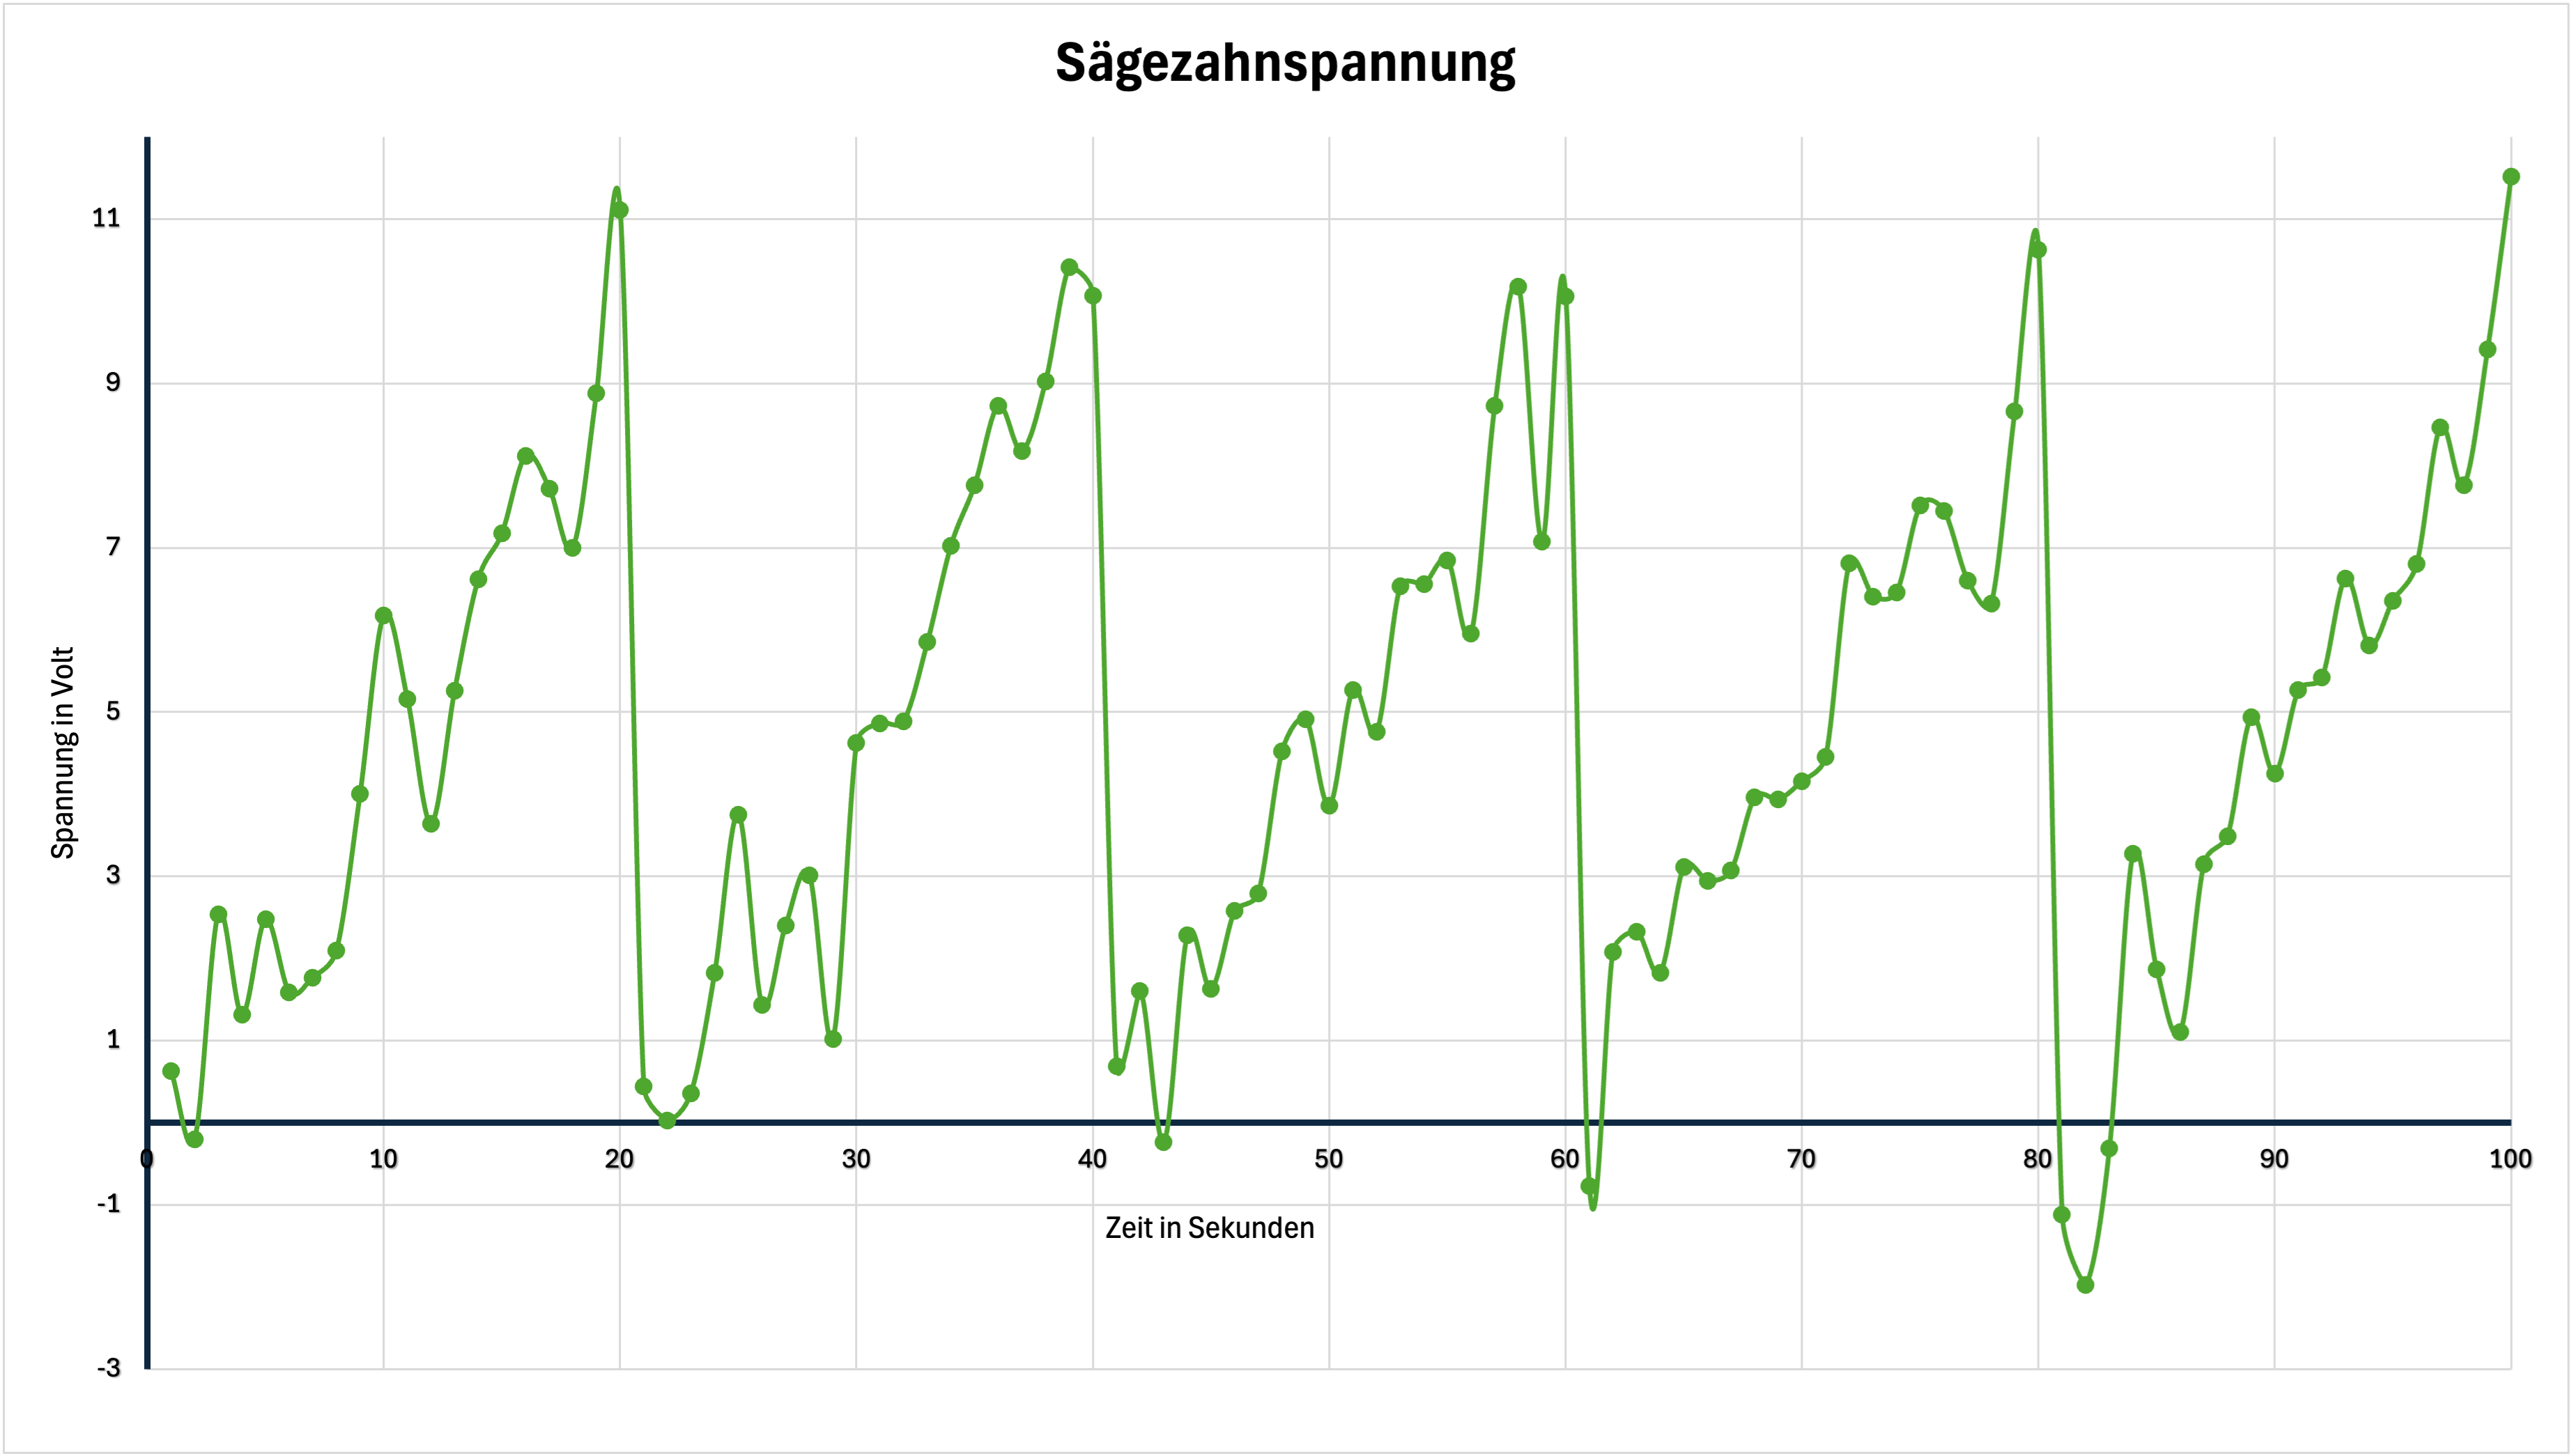
\includegraphics[width=0.8\linewidth]{anlagen/bilder/Graph.png}
        \caption{Verrauschte Sagezahnspannung}
        \label{fig:verrauschte_saegezahnspannung}
    \end{figure}
\end{minipage}\end{lstlisting}

\begin{minipage}[c]{0.45\textwidth}
    \begin{table}[H]
        \centering
        \begin{tabular}{|c|c|}
            \hline
            \textbf{Wert 1} & \textbf{Wert 2} \\
            \hline
            1               & 2               \\
            3               & 4               \\
            \hline
        \end{tabular}
        \caption{Beispiel Tabelle}
        \label{tab:beispiel_tabelle}
    \end{table}
    Dies ist eine Tabelle, in der einige Daten aufgeführt sind.
\end{minipage}
\hfill
\begin{minipage}[c]{0.45\textwidth}
    Es folgt ein Bild, welches eine verrauschte Sägezahnspannung darstellt.
    \begin{figure}[H]
        \centering
        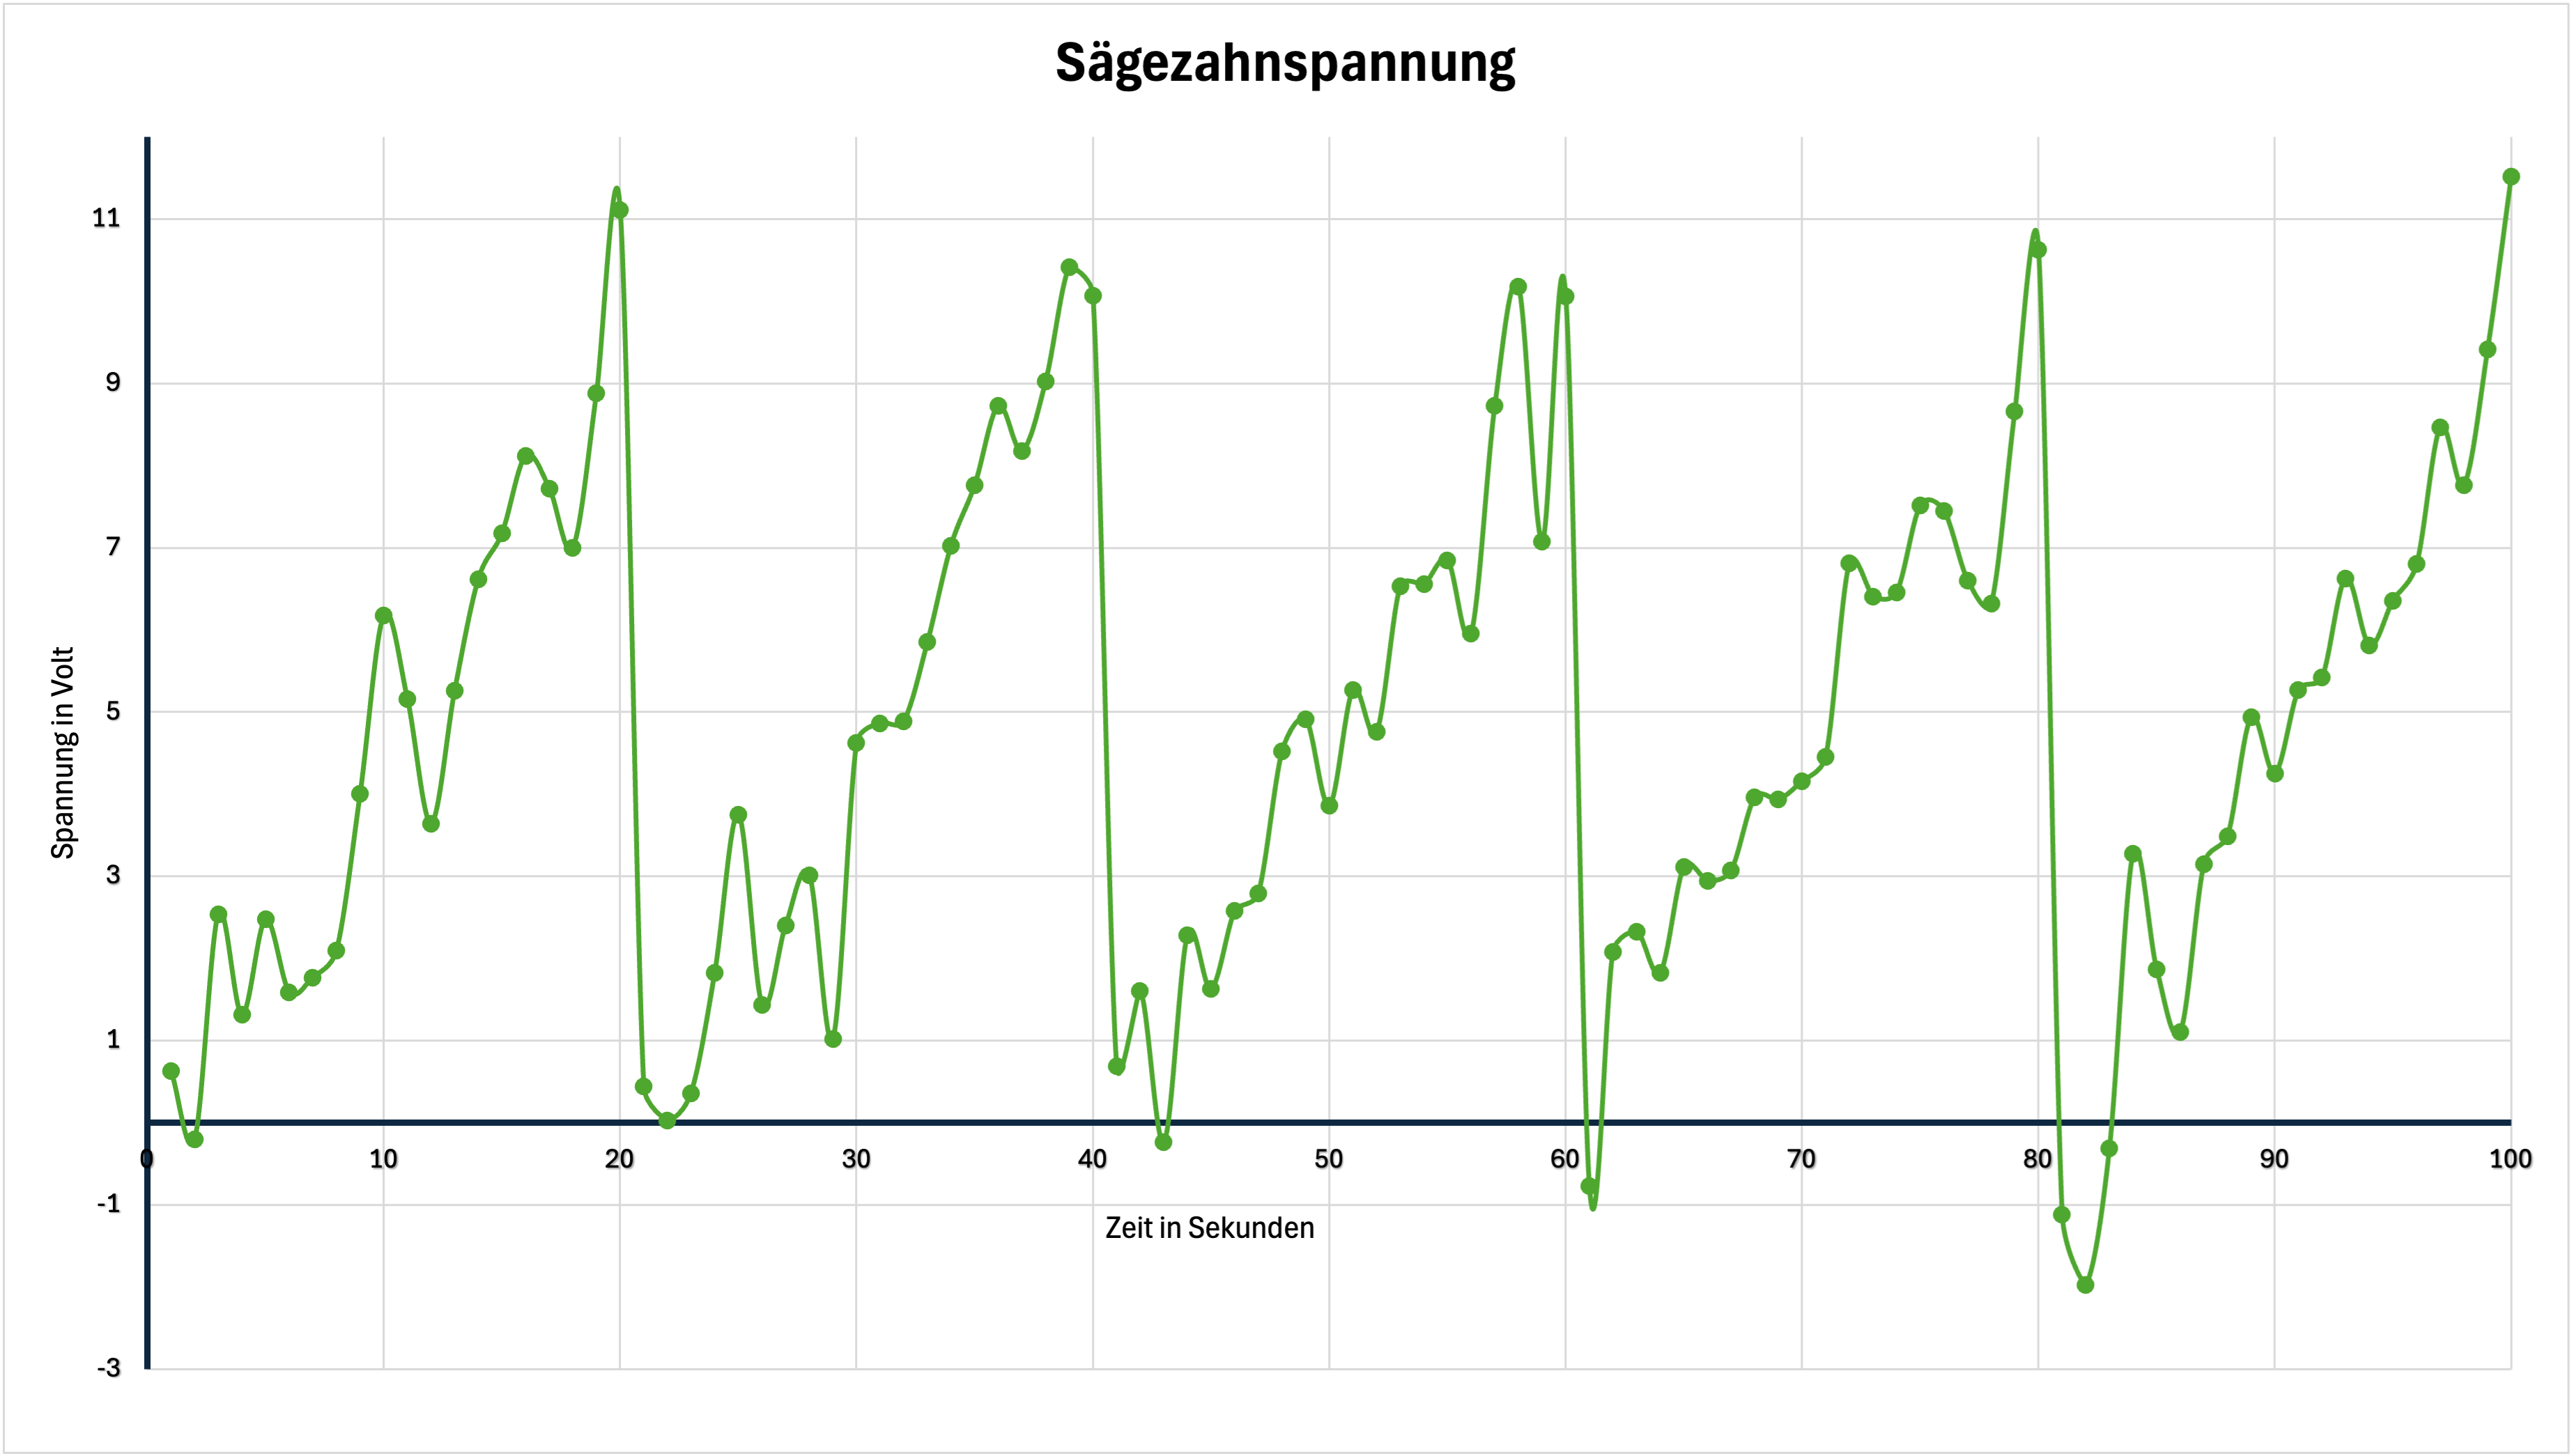
\includegraphics[width=0.8\linewidth]{anlagen/bilder/Graph.png}
        \caption{Verrauschte Sägezahnspannung}
        \label{fig:verrauschte_saegezahnspannung}
    \end{figure}
\end{minipage}

\subsubsection{Parbox}
Mit dem Befehl \textbf{\texttt{\textbackslash parbox[Ausrichtung]\{Breite\}\{Inhalt\}}} kann Text in einer Box platziert werden:
Die Boxen lassen sich mit einem Rahmen anschließen (siehe auch: \autoref{sec:rahmen_und_boxen}).

\begin{lstlisting}[language={[LaTeX]TeX}, basicstyle=\small]
\fbox{\parbox[t]{0.3\textwidth}{Dies ist ein Beispieltext, der in einer Box platziert wurde.}}
\hfill
\parbox[t]{0.3\textwidth}{Dies ist ein zweiter Beispieltext, der in einer Box platziert wurde.}
\hfill
\colorbox{red!20}{\parbox[t]{0.3\textwidth}{Dies ist ein dritter Beispieltext, der in einer Box platziert wurde.}}
\end{lstlisting}

\fbox{\parbox[t]{0.3\textwidth}{Dies ist ein Beispieltext, der in einer Box platziert wurde.}}
\hfill
\parbox[t]{0.3\textwidth}{Dies ist ein zweiter Beispieltext, der in einer Box platziert wurde.}
\hfill
\colorbox{red!20}{\parbox[t]{0.3\textwidth}{Dies ist ein dritter Beispieltext, der in einer Box platziert wurde.}}

